\documentclass[12pt,a4paper]{article}
\usepackage[utf8]{inputenc}
\usepackage{amsthm}
\newtheorem{teorema}{Teorema}[section]
\newtheorem{prop}{Proposição}[section]
\usepackage{amsmath}
\usepackage{amsfonts}
\usepackage{amssymb}
\usepackage[top=3cm, bottom=2cm, left=3cm, right=2cm]{geometry} % geometria da pagina
\usepackage{natbib} 			% Fazer referencias bibliograficas
\usepackage{graphicx}
\usepackage{subfig}
\graphicspath{{figuras/}}
\usepackage{macrosfabbri}
\usepackage{indentfirst}
%\usepackage{url}
\usepackage{hyperref}
\usepackage[brazil]{babel}
\usepackage{epigraph}%entra com epigrafe no inicio das secoes - comando: \epigraph
\usepackage{setspace}%espacamento
\usepackage{transparent}%transparencia da marca d'agua
\usepackage{eso-pic}%incluir marca d'agua
\usepackage{wrapfig}%inserir figura na lateral do texto

%comandos criados por David
\newcommand{\bpi}{\pi}
\newcommand{\y}{{\bf y}}
\newcommand{\C}{{\bf C}}
\newcommand{\marcagua}{\put(0,0){\parbox[b][\paperheight]{\paperwidth}{\vfill\centering{\transparent{0.1}\includegraphics[scale=1.9]{logo-uerj-cinza}}\vfill}}}%inserir a figura da marca d'agua

\setstretch{1.5}%espacamento padrao, mas pode ser alterado durante o texto com esse mesmo comando

\begin{document}

%\AddToShipoutPicture*{\marcagua}
%\input{capa}
%\input{anv-folha-rosto}

\thispagestyle{empty}

\begin{center}
David da Costa de Pinho

\vspace{2 cm}

{\bf Geometria trifocal em reconstrução 3D}
\end{center}

\vspace{2 cm}

\begin{flushright}
\begin{minipage}{.5\textwidth}
\setstretch{1}
Dissertação apresentada, como
requisito parcial para obtenção do título de Mestre, ao Programa de Pós-Graduação em Modelagem Computacional, da Universidade do Estado do Rio de Janeiro. Área de concentração: Visão Computacional.
\end{minipage}
\end{flushright}

\begin{flushleft}
Aprovada em 19 de fevereiro de 2016\\
Banca examinadora:
\end{flushleft}

\vspace{1 cm}

\begin{center}
\begin{tabular}{c}
\hline
Prof. Ricardo Fabbri, Ph.D.\\
Instituto Politécnico do Rio de Janeiro - UERJ\\\\\\

\hline
Prof$^{\,\,\text{a}}$. Lis Ingrid Roque Lopes Custódio, D.Sc.\\
Instituto Politécnico do Rio de Janeiro - UERJ\\\\\\

\hline
Prof. Nelson Violante-Carvalho, Ph.D.\\
Universidade Federal do Rio de Janeiro
\end{tabular}
\end{center}

\vspace{3 cm}

\begin{center}
Nova Friburgo\\
2016
\end{center}




\pagestyle{empty}

\begin{center}
{\bf AGRADECIMENTOS}
\end{center}

\vspace{1 cm}

Agradeço aos senhores José Saulo Pereira de Pinho, Vilma Nadir Mozer, Pablo Mozer de Pinho, Patrick Mozer de Pinho e Jussara dos Santos por todo o apoio logístico como transporte, estadia e alimentação, muito importantes para a manutenção do curso de Pós-Graduação e confecção da dissertação, já que não recebi apoio financeiro de qualquer órgão de fomento a pesquisas acadêmicas.

Agradeço ao prof. Ricardo Fabbri por se disponibilizar como orientador, disponibilizar máquina de uso pessoal e espaço em seu laboratório. Por, várias vezes, priorizar minha pesquisa em detrimento de funções burocráticas no âmbito do IPRJ e até mesmo em detrimento de suas pesquisas pessoais. Por transmitir suas reflexões e filosofia acerca de estudos acadêmicos. 

Agradeço ainda ao prof. Ricardo Carvalho de Barros pelos ensinos em álgebra linear que foram cruciais em pelo menos três momentos durante minhas investigações teóricas.
\newpage
\quad\\
\vspace{21 cm}

\noindent Na falta de uma interpretação geométrica, um grande conjunto de equações algébricas pode ser tão informativo quanto um bloco de códigos de programação.

\begin{flushright}
{\it Stephen Maybank}
\end{flushright}

\newpage
\begin{center}
{\bf RESUMO}
\end{center}

\vspace{1 cm}

\begin{center}
\begin{minipage}{1\textwidth}
\setstretch{1}
\noindent PINHO, D. C. {\it Geometria trifocal em reconstrução 3D.} Dissertação (Mestrado em Modelagem Computacional) - Instituto Politécnico do Rio de Janeiro, Universidade do Estado do Rio de Janeiro, Nova Friburgo, 2016.
\end{minipage}
\end{center}

\vspace{1 cm}

\begin{center}
\begin{minipage}{1\textwidth}
\setstretch{1}
\qquad Neste trabalho nós investigamos alguns benefícios na utilização da geometria trifocal aplicada em sistemas de reconstrução 3D multifocal e estimação de modelos de múltiplas câmeras, em oposição à utilização da geometria epipolar com pares de câmeras. Apresentamos a interpretação e o detalhamento matemático dos pontos mais importantes de dois artigos recentes e essenciais, objetivando resolver problemas trifocais de estrutura de curvas no futuro. Equanto um deles mostra a aplicação do quatérnion de Hamilton e das bases de Gr\"obner para a cálculo da pose de uma câmera dadas estruturas correspondentes 3D--2D, o outro é a abordagem mais eficiente computacionalmente (até a presente data) na reconstrução das câmeras num sistema trifocal. Os primeiros capítulos e os apêndices apresentam as teorias básicas sobre geometria projetiva, álgebra linear e geometria algébrica necessárias ao avanço das pesquisas no campo da reconstrução 3D trifocal e multifocal e sistemas de determinação de estruturas a partir do movimento.
\end{minipage}
\end{center}
 
\vspace{1 cm}

\begin{flushleft}
Palavras-chave: Visão computacional. Reconstrução 3D. Geometria trifocal. Bases de Gr\"obner. 
\end{flushleft}

\newpage
\begin{center}
{\bf ABSTRACT}
\end{center}

\vspace{1 cm}

\begin{center}
\begin{minipage}{1\textwidth}
\setstretch{1}
\noindent PINHO, D. C. {\it Trifocal geometry in 3D reconstruction.} Dissertação (Mestrado em Modelagem Computacional) - Instituto Politécnico do Rio de Janeiro, Universidade do Estado do Rio de Janeiro, Nova Friburgo, 2016.
\end{minipage}
\end{center}

\vspace{1 cm}

\begin{center}
\begin{minipage}{1\textwidth}
\setstretch{1}
\qquad In this work we present some advantages using trifocal geometry applied to transfers and cameras computation, to confront using epipolar geometry in three view system. There are the detailed exposition of the most important mathematical tools in two papers. While one of them shows the Hamilton's Quaternions and Gr\"obner Bases applications to one camera's computation, the other one is the most efficient approach (at least until 2006) to trifocal system reconstruction of cameras. It's available in the first chapters and appendix, the basic theory about Projective Geometry, Linear Algebra and Algebraic Geometry useful to dissertation learnning.
\end{minipage}
\end{center}
 
\vspace{1 cm}

\begin{flushleft}
Keywords: Computer vision. 3D reconstruction. Trifocal geometry. Gr\"obner bases. 
\end{flushleft}

\newpage

\tableofcontents

\newpage
\pagestyle{headings}
\section{Introdução}
A Visão Computacional é uma área de pesquisa que se ocupa em utilizar imagens em 2D de um cenário, obtidas de uma ou mais câmeras digitais para produzir uma construção virtual em 3D, ou extrair qualquer outro tipo de informação útil como o cruzamento de informações entre imagens. A captação da geometria 3D de um cenário a partir de imagens produzidas por câmeras, analisando a disparidade entre elementos correspondentes nessas imagens, é chamada de visão {\it estereoscópica}, da qual a visão computacional se utiliza para desenvolver modelos adequados à descrição geométrica tanto da cena 3D em questão como das câmeras que fazem a projeção da cena na imagem 2D.  

\begin{figure}[!htb]
\centering
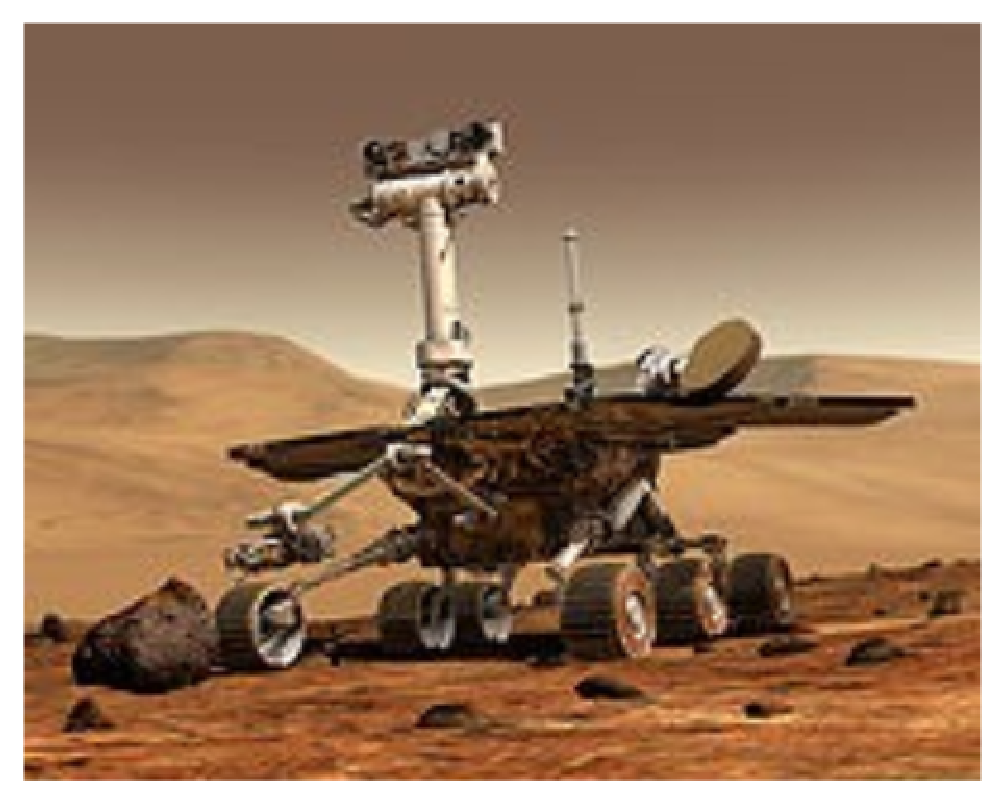
\includegraphics[scale=.5]{mars-rover}
\caption{{\it O maior passo no uso de visão computacional em pesquisas interplanetárias foi dado na missao NASA/JPL Mars Exploration Rover (MER).}}
\label{fig.mars-rover}
\end{figure}

A geometria projetiva é a principal teoria matemática usada em visão computacional tridimensional. Com a introdução de algumas definições e conceitos, a geometria projetiva pode ser estudada em termos de álgebra linear, onde tal abordagem traz alguns benefícios de modelagem e é amplamente utilizada por pesquisadores dessa área, mas também possui algumas limitações. Em pesquisas mais recentes, verificou-se a eficácia do uso de técnicas de geometria algébrica em resoluções de sistemas de equações polinomiais, oriundos de problemas de visão computacional 3D. Mais recentemente ainda, \citep{tese-fabbri} introduziram uma abordagem em termos de geometria diferencial, onde é possível aplicar o cálculo diferencial trabalhando diretamente com as equações algébricas. Essa abordagem permite um maior poder de modelagem matemática e computacional do espaço tridimensional através das imagens.


\subsection*{Motivação}
As motivações para a pesquisa estão ligadas às suas aplicações em diversas áreas. A extração de informação da geometria 3D de um ambiente pode, por exemplo, ser utilizada na determinação da orientação e posição de veículos autônomos, para que os mesmos identifiquem a trajetória para os seus objetivos considerando a possibilidade de obstáculos. Um exemplo famoso, segundo \citep{mars-rover}, é a aplicação em pesquisas interplanetárias onde foram usados algoritmos de visão computacional em veículos de exploração de Marte (Mars Exploration Rover - MER, em inglês), observado na figura \ref{fig.mars-rover}.


Uma aplicação mais recente foi a reconstrução virtual de objetos, estátuas ou monumentos de valor histórico e cultural que tenham sido destruídos pela ação do tempo ou do homem (possivelmente em guerras), através da aquisição de imagens em acervos ou na internet. Um exemplo é o Museu de Mosul {\footnote{Outros exemplos podem ser encontrados em http://www.projectmosul.org/}}, no Iraque, atacado pelo 
Estado Islâmico em 2015, que teve algumas de suas obras reconstruídas como podemos visualizar na figura \ref{fig.mossul}.

\begin{figure}[!htb]
\centering
\subfloat{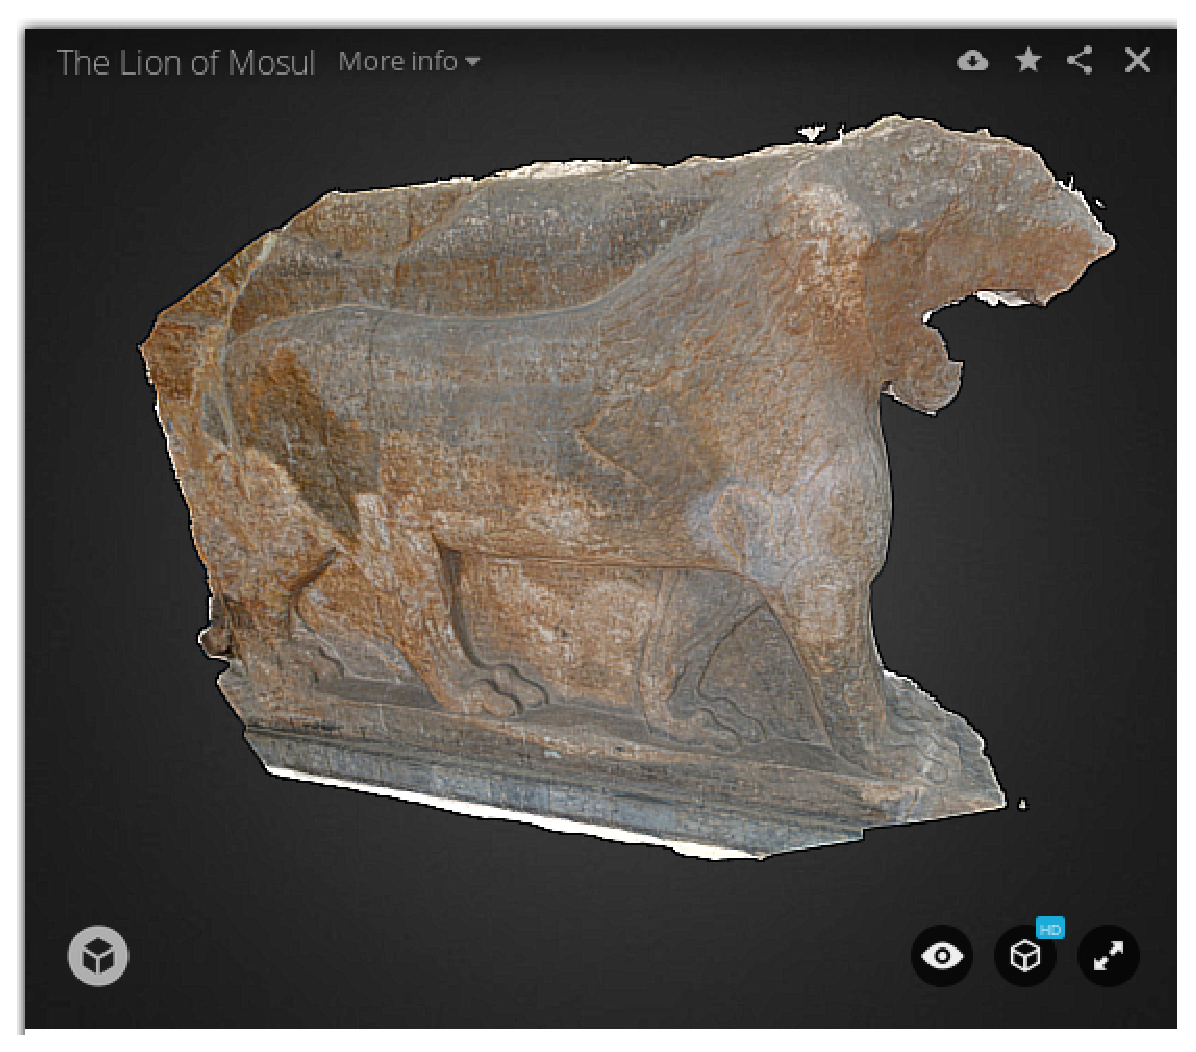
\includegraphics[scale=.385]{leao-mosul}}
\quad
\subfloat{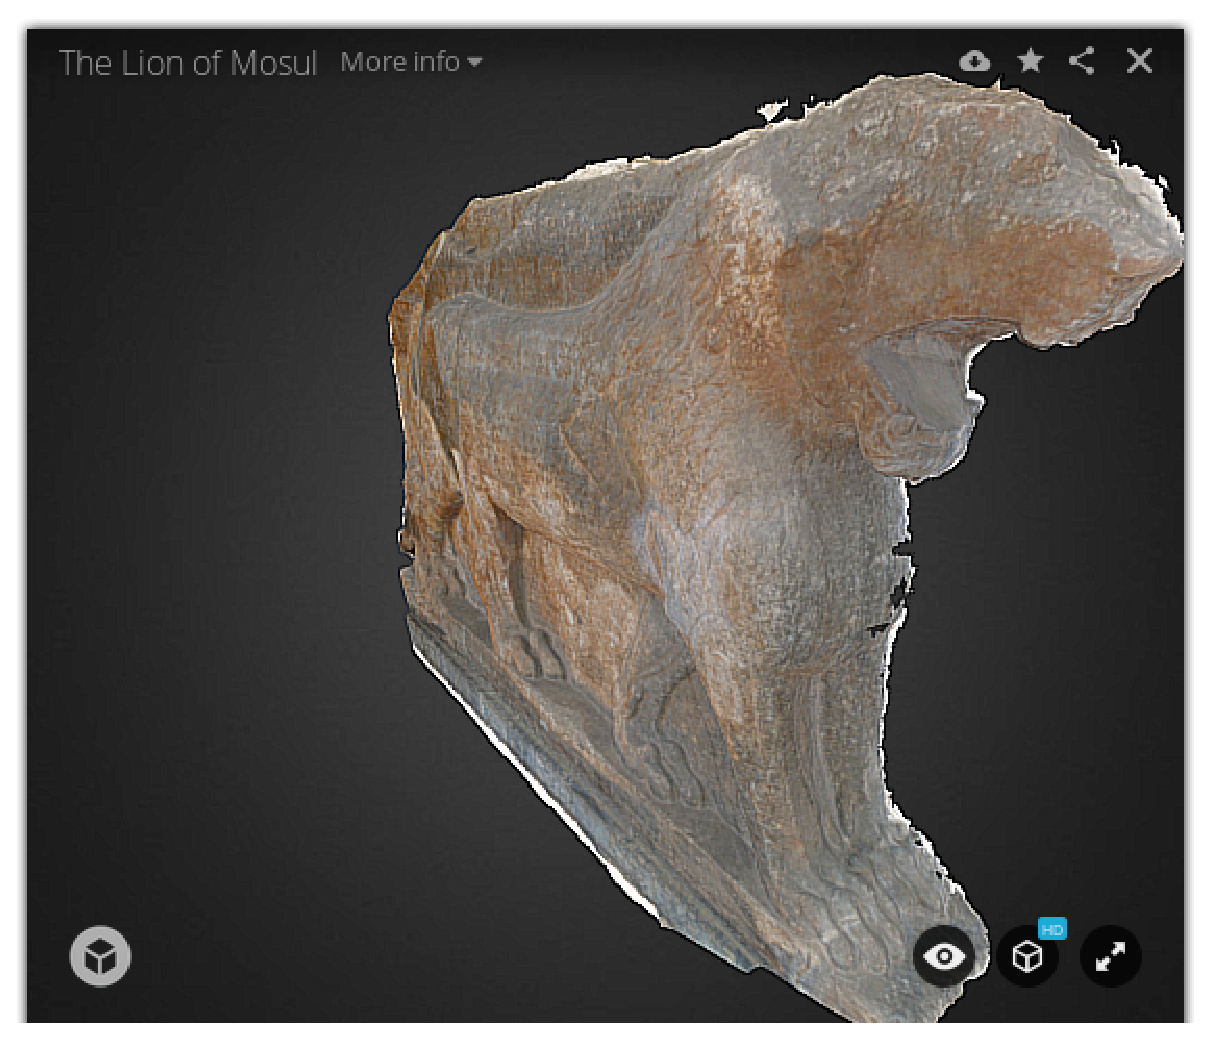
\includegraphics[scale=.385]{lion-mosul-2}}
\caption{{\it A reconstrução do Leão de Mosul, um dos artefatos destruídos por extremistas religiosos em 2015 no Iraque.}}
\label{fig.mossul}
\end{figure}

As aplicações de visão computacional são bastante variadas, com pesquisas em outras áreas como astronomia, medicina e química. Para se ter uma ideia, \citep{ballard-82} já apresentavam imagens e tabelas com resumos de aplicações em oito áreas diferentes no início dos anos 1980.  

Novos avanços em reconstrução 3D vêm sendo realizados constantemente como observamos em \citep{fabbri-drawing}, que apresentam uma abordagem para a reconstrução de um esboço 3D (3D drawing em inglês) de uma cena. Isto é, um conjunto de fragmentos de curvas em 3D interligadas de forma que preserve suas relações espaciais, capturadas em forma de gráficos a partir de um grande conjunto de dados multifocal. A ideia base é aprimorar uma abordagem anterior (3D curve sketch) divulgada pelos mesmos autores, \citep{fabbri-sketch}, conforme exemplo visualizado na figura \ref{fig.drawing}.
\begin{figure}[!htb]
\centering
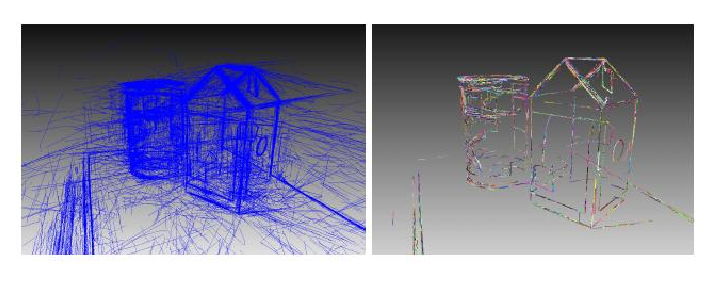
\includegraphics[scale=1.1]{3D-drawing}
\caption{{\it Uma comparação visual: à esquerda os resultados com o 3D curve sketch e à direita os resultados após o aprimoramento com 3D drawing. Repare na redução significante de outliers sem prejuízo do esboço da superfície.}}
\label{fig.drawing}
\end{figure}

A maioria dos métodos de reconstrução não utilizam geometria diferencial de curvas, mas se baseiam em correlacionar pontos de interesse através das imagens e produzem uma desorganizada nuvem de pontos em 3D, figura \ref{fig.medusa}. Tais métodos obtêm sucesso em ambientes controlados, com cenas em larga escala e imagens ricas em textura, mas não podem ser aplicados em configurações gerais. Não podem reconstruir superfícies suaves e homogêneas nem suas fronteiras devido a esparsidade de pontos de interesse, como também não podem reconstruir regiões que se alteram drasticamente com a mudança de luz ambiente. Exemplos de imagens sujeitas a essas limitações são dados na figura \ref{fig.carro-objeto-curvo}.
\begin{figure}[!htb]
\centering
\subfloat{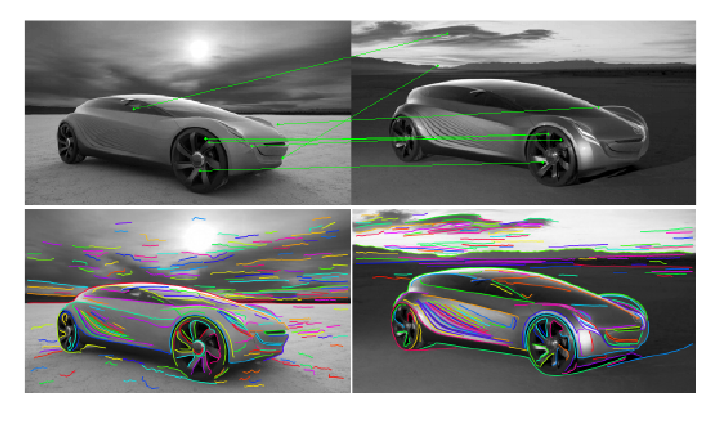
\includegraphics[scale=.76]{carro}}
\quad
\subfloat{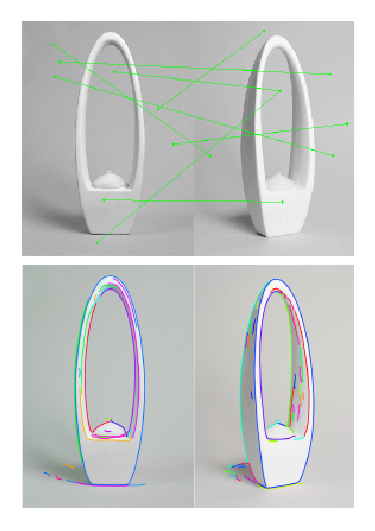
\includegraphics[scale=.6]{objeto-curvo}}
\caption{{\it Exemplos de objetos que não podem ser reconstruídos através da abordagem tradicional usando pontos de interesse e a geometria epipolar.}}
\label{fig.carro-objeto-curvo}
\end{figure}  
Daí são utilizadas outras técnicas de melhoramento dos resultados, como a Interpolação de Pontos e Texturização, mas que não fornecem um resultado plenamente satisfatório. Podemos ver as fases desse processo em um exemplo no conjunto de imagens na figura\ref{fig.medusa}.

Portanto, ainda é necessário que se continuem as pesquisas em visão computacional, e o presente trabalho tem a finalidade de, primeiramente, detalhar as abordagens de artigos recentes na busca de novas combinações de ferramentas matemáticas que possam melhorar as atuais abordagens e atenuar o esforço computacional. Segundo, a verificação dos benefícios obtidos com o uso da geometria trifocal em transferência de pontos e reconstrução 3D em comparação com a geometria epipolar (mais usada atualmente), tudo com o objetivo de auxiliar na construção de uma nova abordagem usando geometria diferencial multifocal em condições realísticas.

\begin{figure}[!htb]
\centering
\subfloat{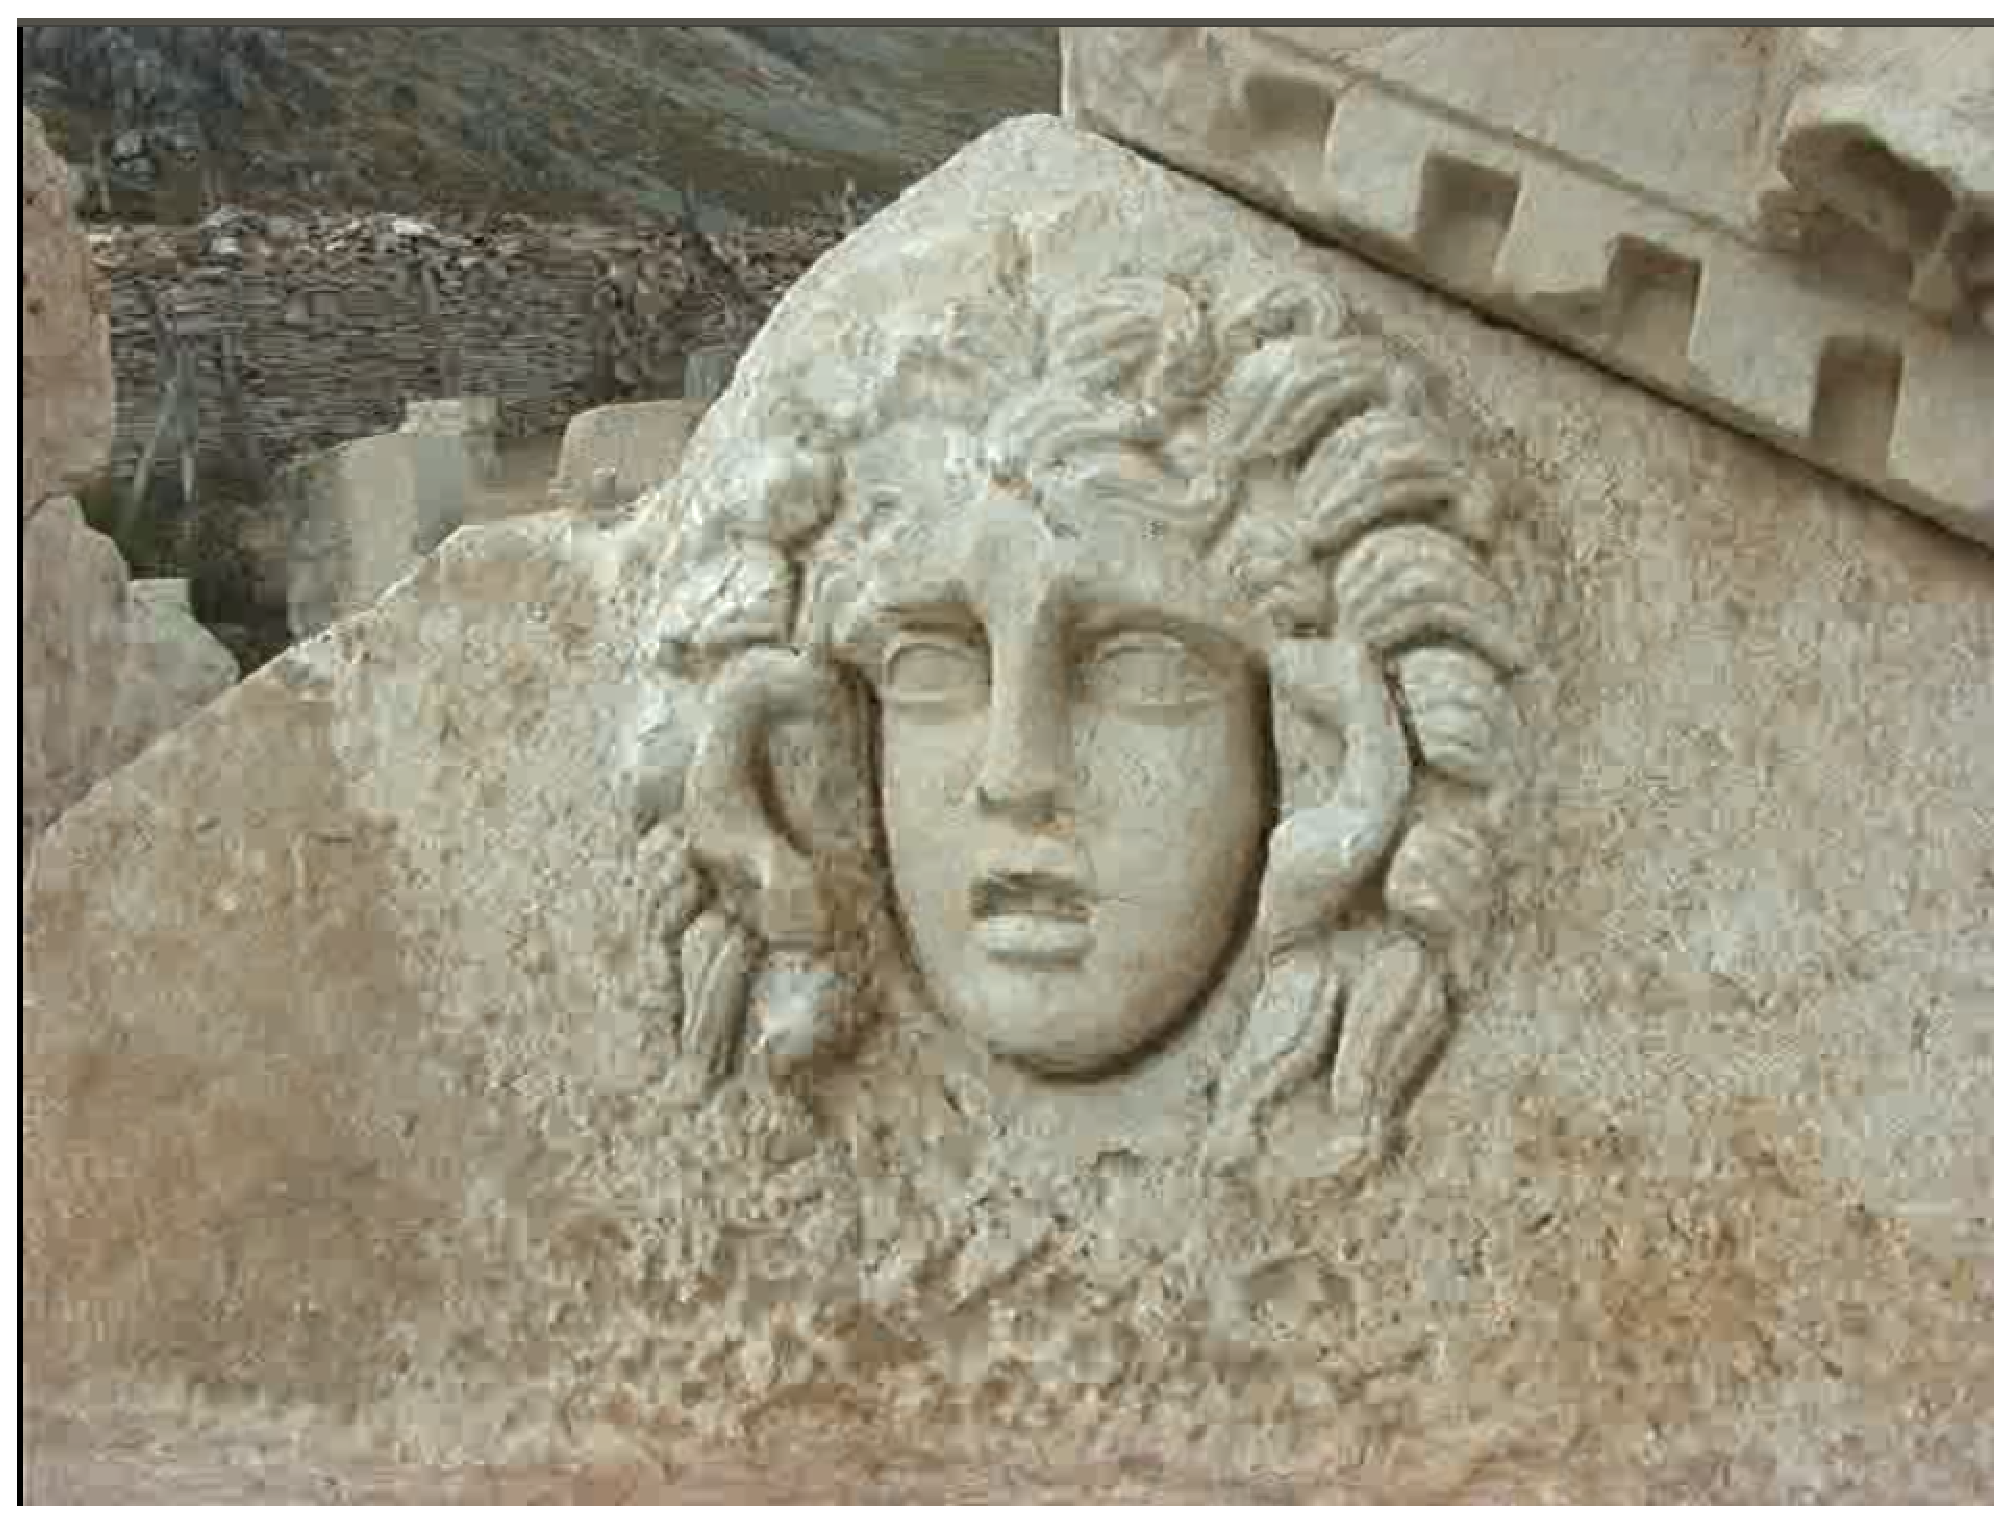
\includegraphics[scale=.2]{medusa1}}
\quad
\subfloat{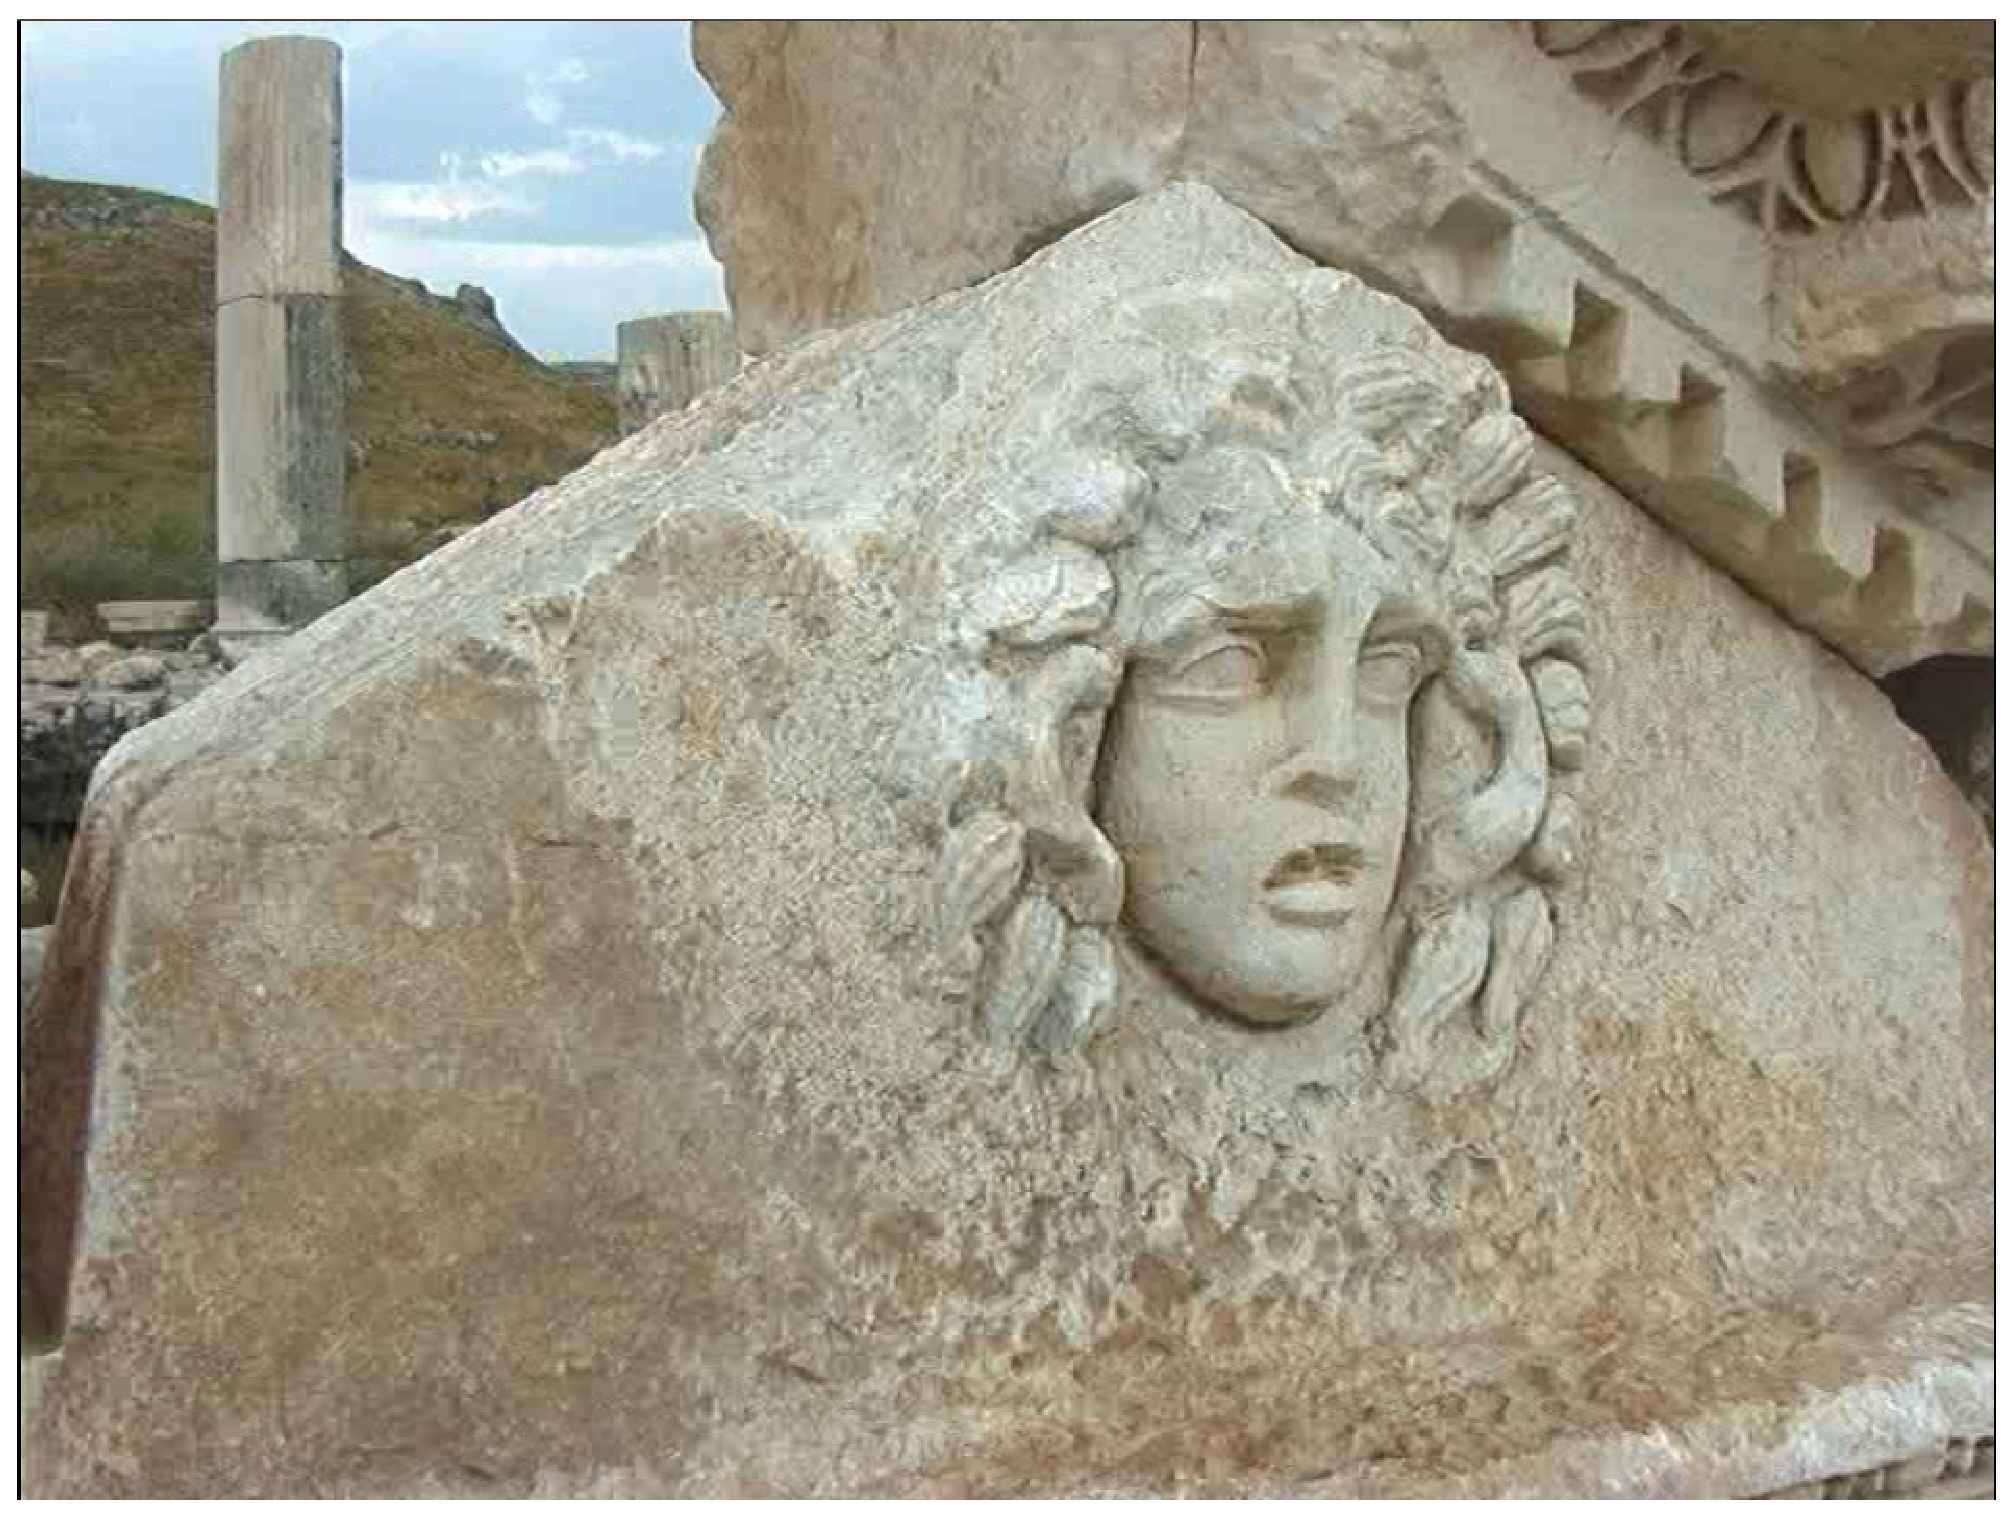
\includegraphics[scale=.2]{medusa2}}
\\
\subfloat{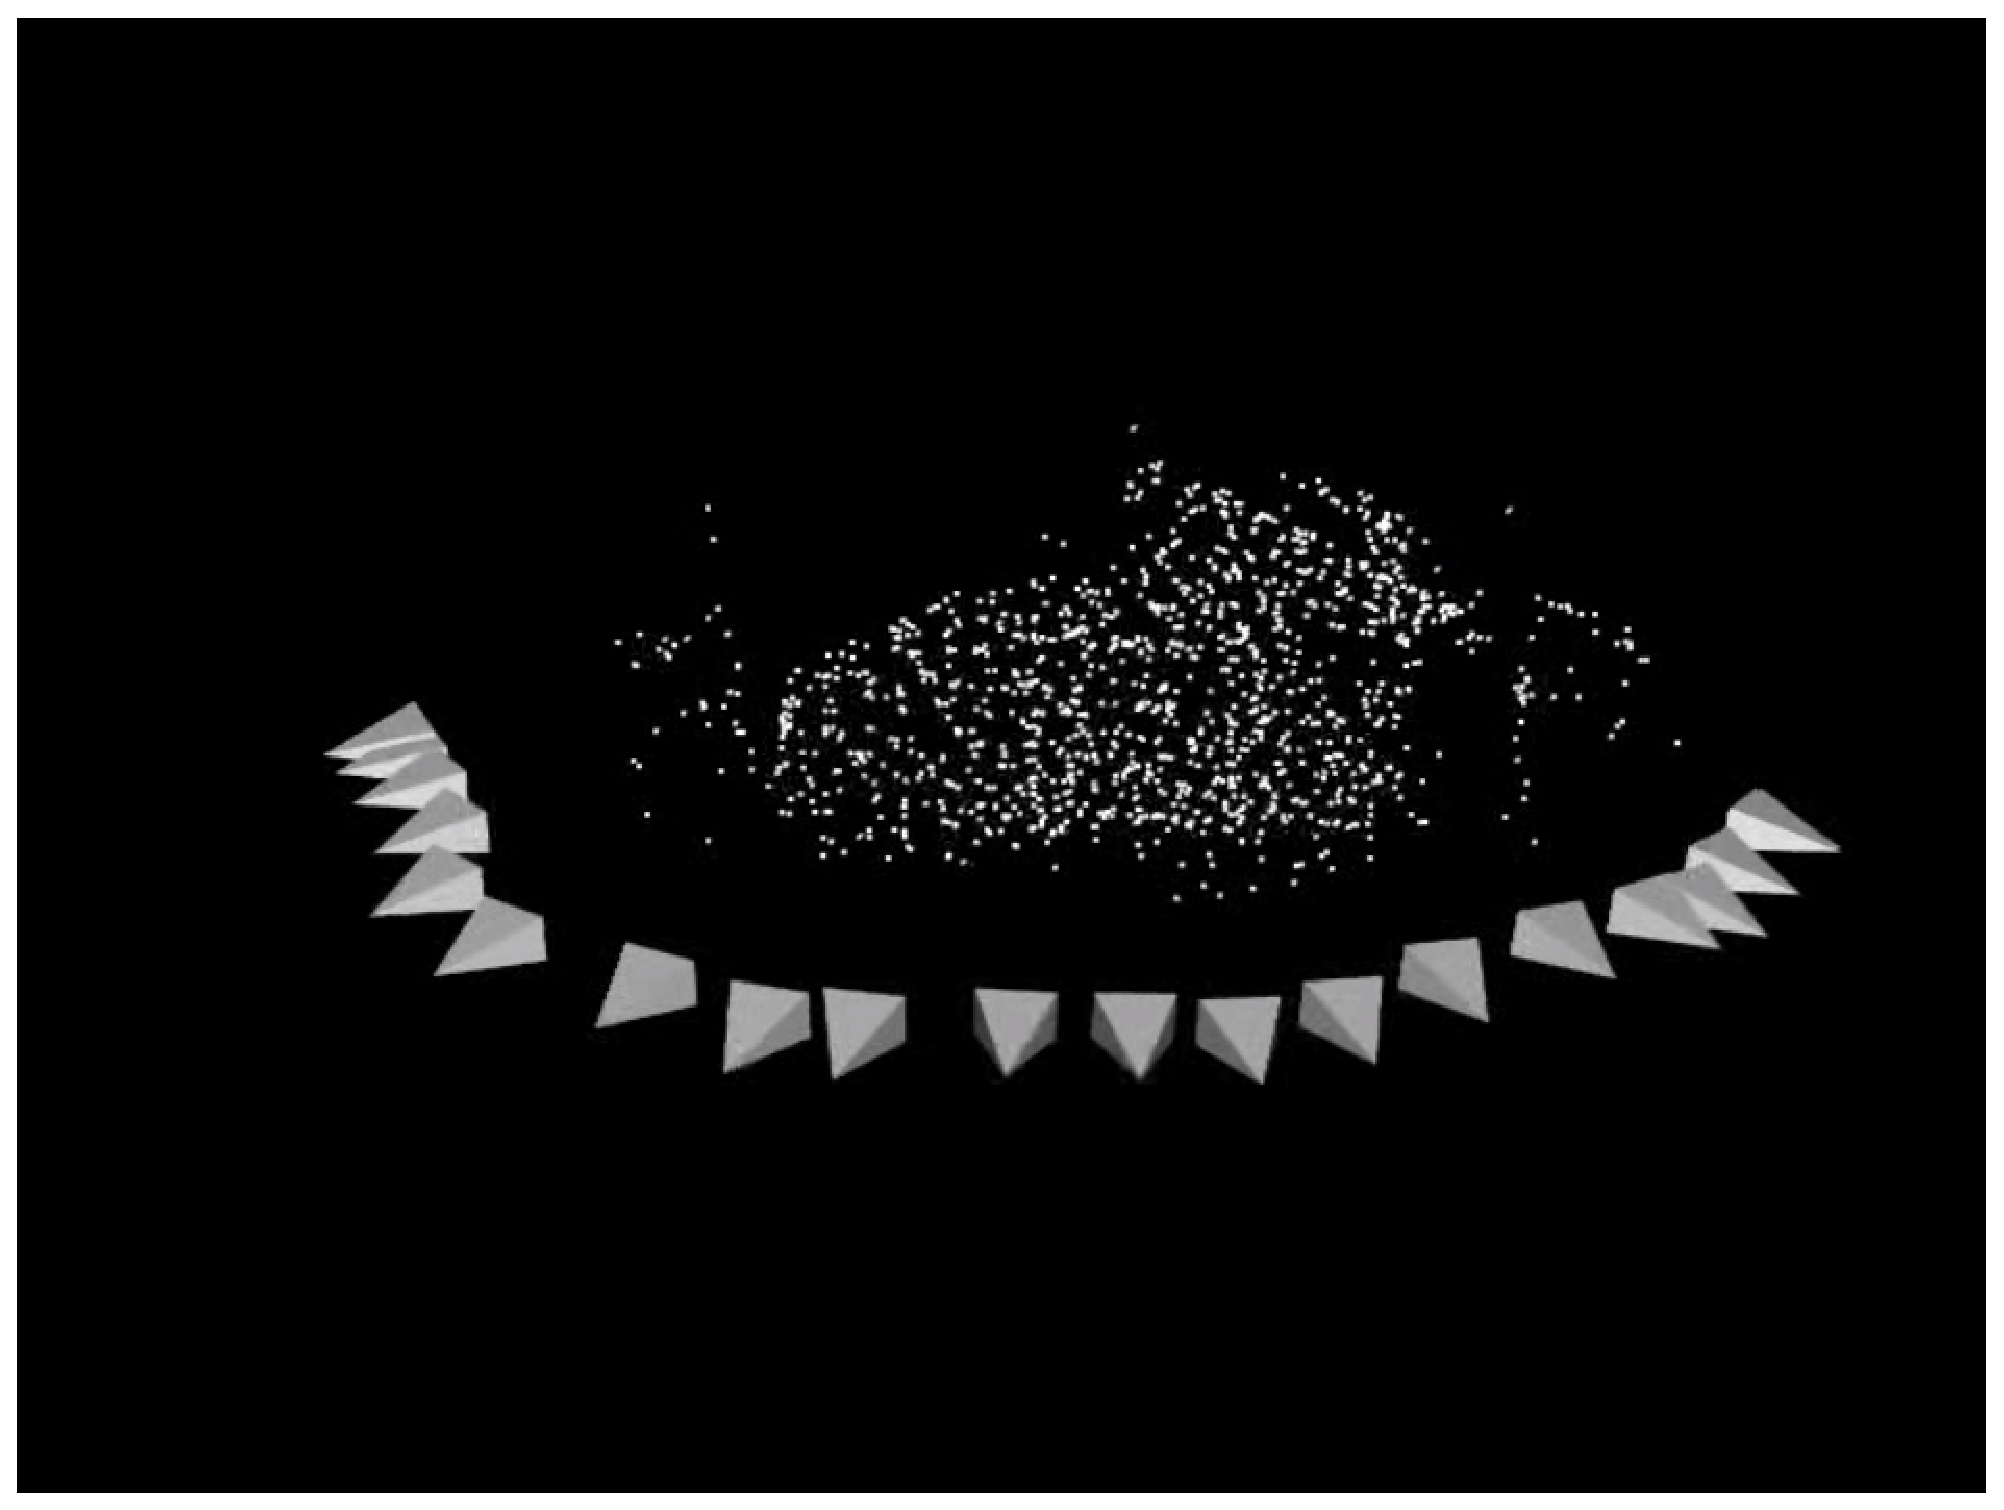
\includegraphics[scale=.2]{nuvem1}}
\quad
\subfloat{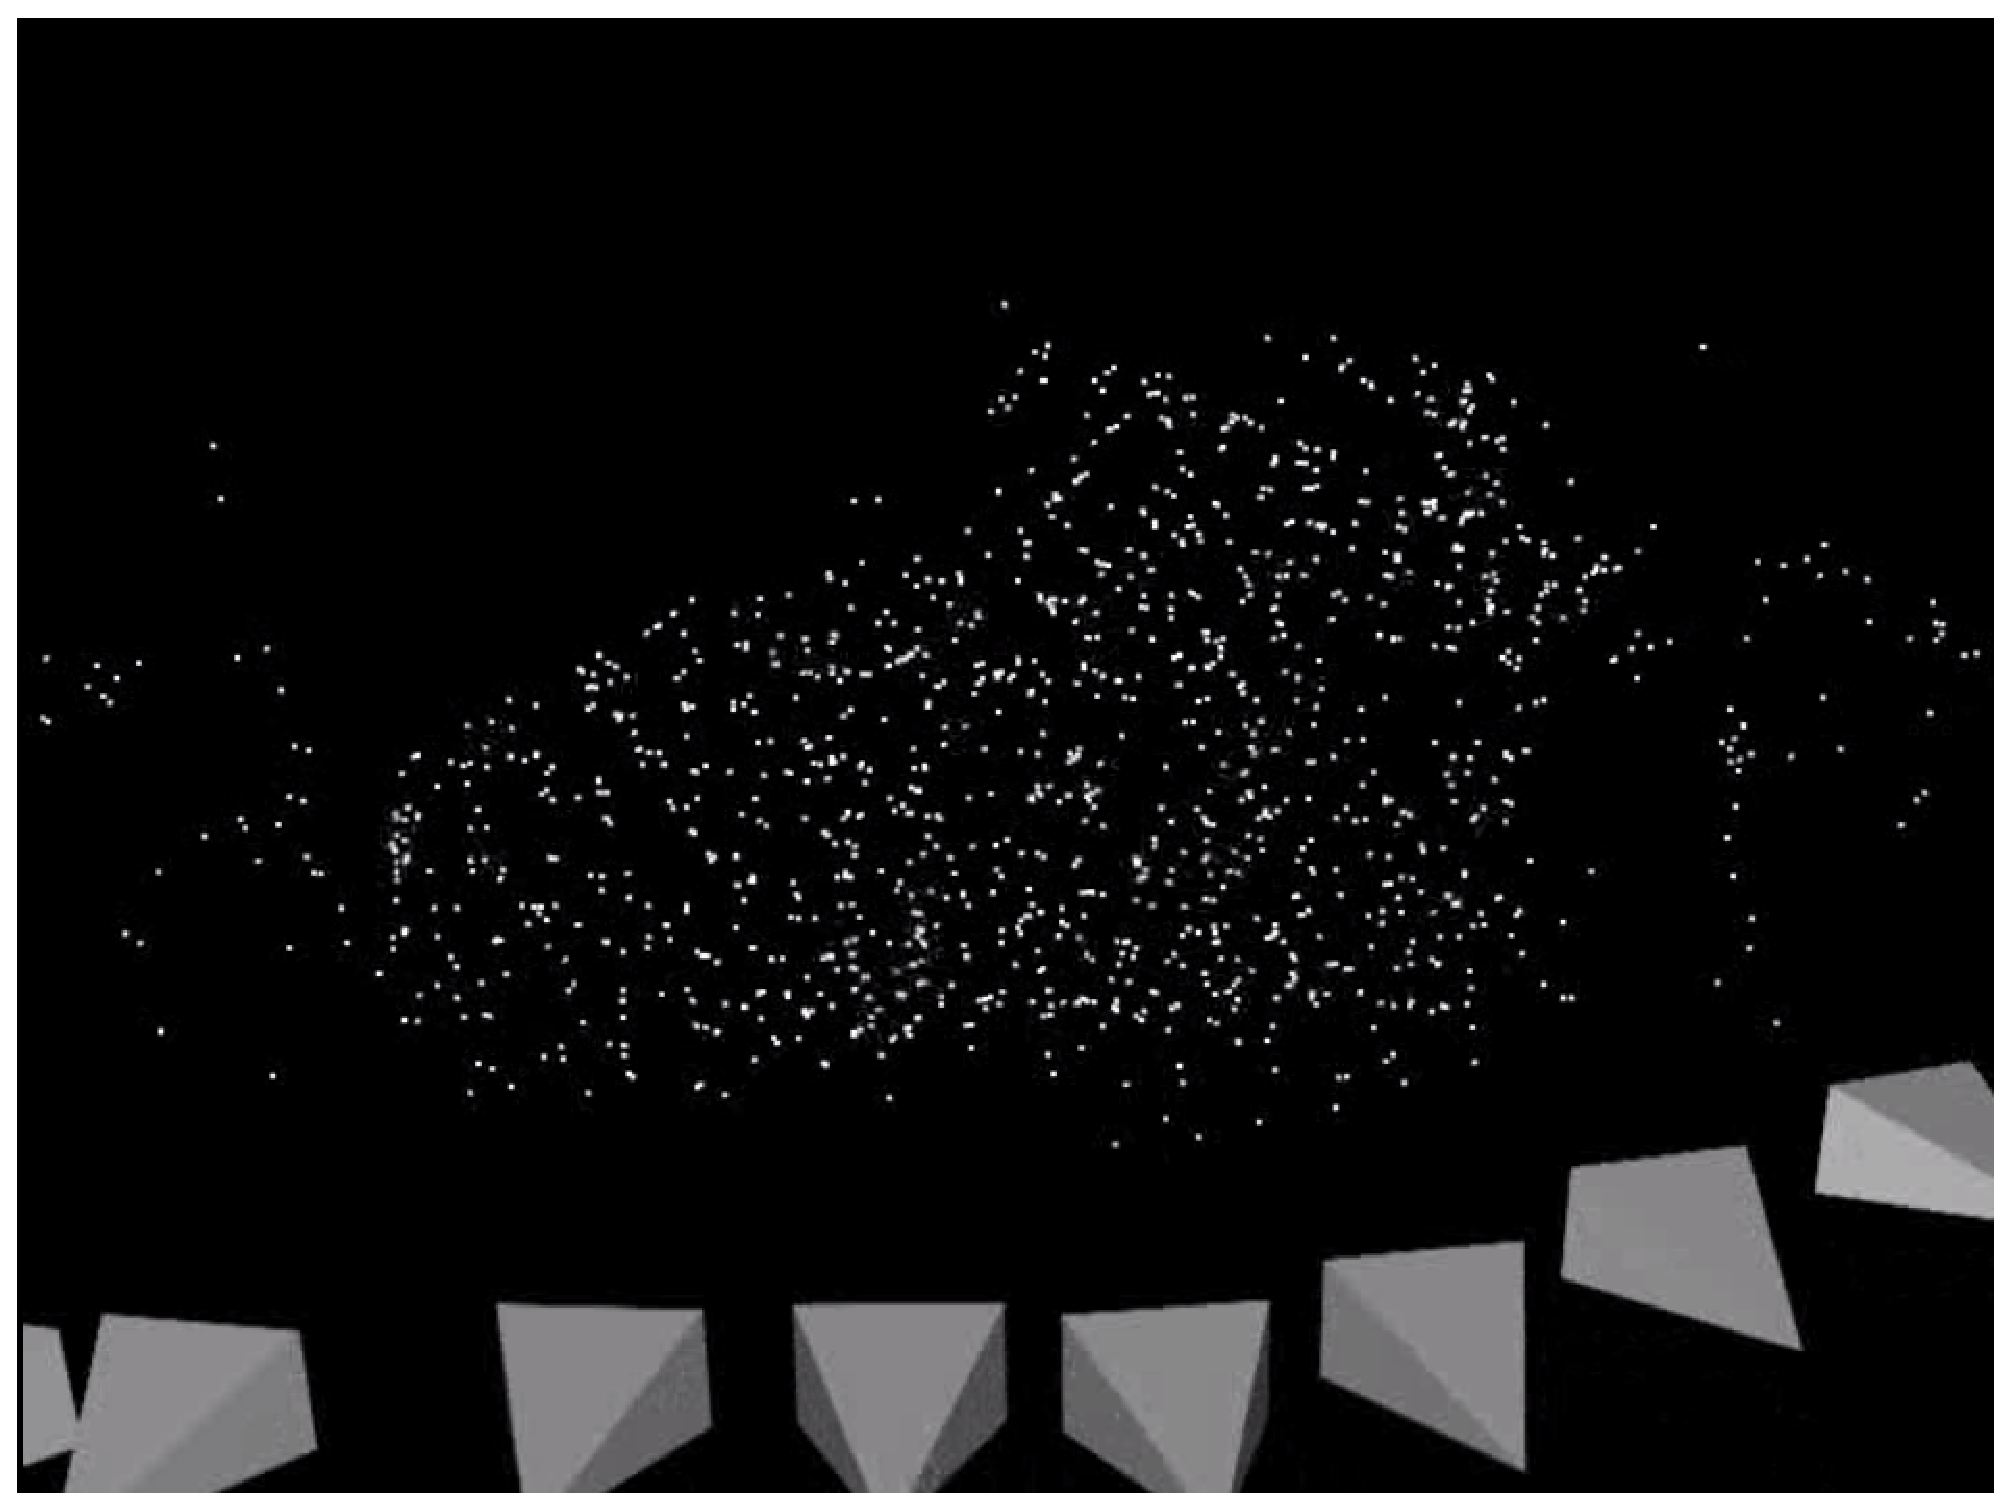
\includegraphics[scale=.2]{nuvem2}}
\\
\subfloat{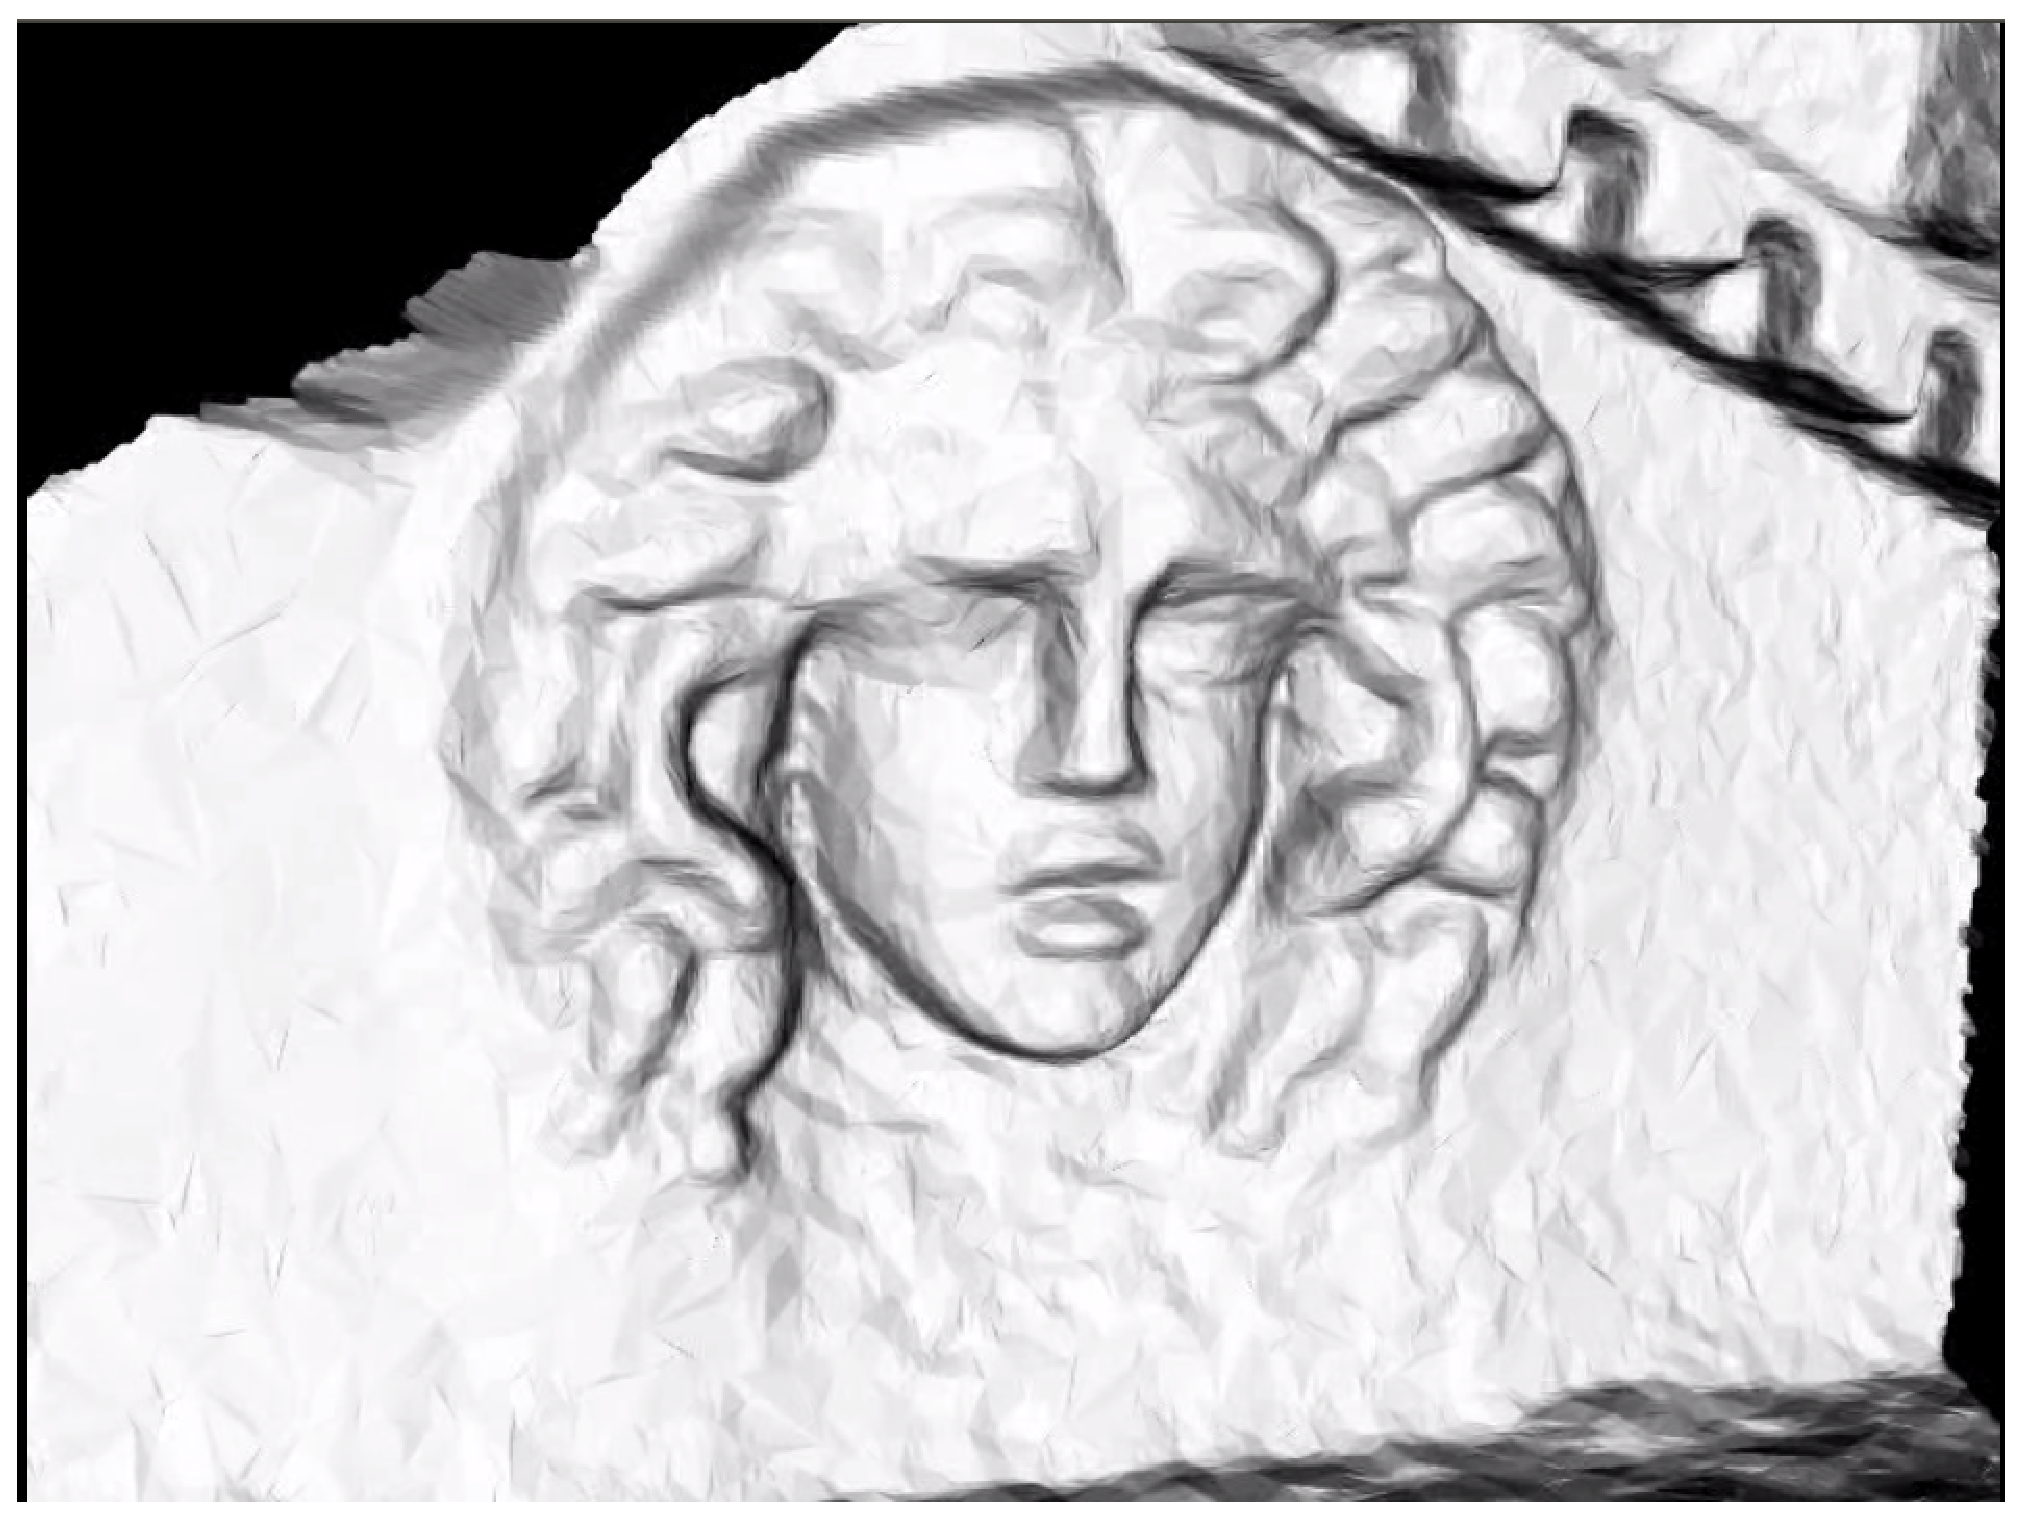
\includegraphics[scale=.2]{texturizacao2}}
\quad
\subfloat{\includegraphics[scale=.2]{texturizacao-realmente}}
\caption{{\it Em cima, duas imagens extraídas de um vídeo (utilizado em reconstrução 3D) da estátua da Meduza. No meio, a nuvem de pontos obtida após a reconstrução 3D juntamente com as posições da câmera. Em baixo, aplicação de interpolação de pontos e texturização.}}
\label{fig.medusa}
\end{figure}

\subsection*{Visão geral e objetivos}

A seção \ref{sec.geo-1-2-cam} engloba a teoria básica de geometria projetiva utilizada em visão computacional 3D, com abordagens em termos de álgebra linear e usando o tipo de notação mais difundido entre pesquisadores da área. Além dos conceitos básicos, também são apresentados alguns conceitos e definições um pouco mais avançados indispensáveis ao entendimento das demais seções da dissertação, tudo com a finalidade de facilitar a compreensão do leitor sem a necessidade de consulta em outras publicações. Em seguida, há a apresentação da geometria epipolar, num sistema de visão estéreo com duas câmeras, bem como extração da matriz fundamental e a reconstrução das câmeras, usando essa abordagem bifocal que é mais comum do que a abordagem trifocal.

Na seção \ref{sec.astrom} temos o detalhamento de um artigo recente e representativo para a reconstrução de uma câmera a partir de objetos geométricos em 3D e suas respectivas imagens em 2D, \citep{bib:kuang}. A importância dessa publicação se verifica na utilização do quatérnion de Hamilton para a parametrização da matriz de rotação da câmera, pois desta forma a matriz que possui nove componentes é parametrizada com apenas três variáveis. Outra vantagem é utilização das Bases de Gr\"obner e da matriz de Ação para solução computacional de sistemas de equações polinomiais de grau elevado e com muitas variáveis.

A geometria trifocal e suas características são abordadas na seção \ref{sec.geo-tri}, juntamente com a descrição dos benefícios do uso dessa geometria num sistema com três câmeras em comparação com uso da geometria epipolar entre cada par de câmeras. Após as comparações são apresentados métodos para a extração das matrizes fundamentais e métodos de reconstrução das câmeras a partir do tensor trifocal.  

Na seção \ref{sec.nister} há o detalhamento matemático da abordagem mais eficiente, até a presente data, para a reconstrução 3D das câmeras num sistema trifocal, \citep{2503343}. O artigo é bastante denso, com 25 teoremas, e apresenta a reconstrução de duas câmeras num sistema bifocal utilizando uma intrincada rede de conhecimentos de geometria projetiva. Depois da reconstrução das duas primeiras câmeras, é utilizada a reconstrução 3D de pontos para a reconstrução da terceira câmera, num procedimento similar ao apresentado na seção \ref{sec.astrom}, ou seja, os dois artigos quase se complementam. Esse trabalho deixa bem clara a dificuldade de se realizar a reconstrução num sistema com três imagens de quatro pontos 3D numa cena.

No apêndice \ref{sec.Apen-A} são fornecidas ferramentas de álgebra linear acompanhadas de algumas definições mais restritas à assimilação da dissertação. No apêndice \ref{sec.geo-algebrica} há uma breve introdução aos conceitos básicos de geometria algébrica seguidos da apresentação (informal e em termos de exemplos) de uma teoria para resolução de sistemas de equações polinomiais com várias variáveis.


%\section{Geometria de Uma e Duas Câmeras}

\subsection{Notação Básica de Geometria Projetiva}

Nesta seção, faremos uma breve introdução aos conceitos básicos de Geometria Projetiva e usaremos a notação contida em (citar hartley), por ser o tipo de notação mais difundido entre pesquisas de visão computacional. Para uma abordagem mais profunda do assunto o leitor pode pesquisar o referido autor.  

\subsubsection{O Espaço Projetivo em Duas Dimensões}



$\Longrightarrow$ A Reta


Sabemos que uma reta no plano $\mathbb{R}^{2}$ pode ser representada pela equação $a\,x+b\,y+c=0$, onde a reta fica perfeitamente determinada pelos valores das constantes $a,b,c$. Desta forma, podemos representar retas através de vetores, e assim a reta $a\,x+b\,y+c=0$ seria representada por $(a,b,c)^T \in \mathbb{R}^{3}$, utlizando o símbolo em negrito $\lightrgb$ para indicar tal vetor escrito em coluna, por padrão. Portanto $\lightrgb = (a,b,c)^T$. Note que a relação entre uma dada reta e o seu respectivo vetor não é biunívoca, pois o vetor $k\,(a,b,c)^T$, tal que $k \in \mathbb{R}$, representa a reta $k\,a\,x+k\,b\,y+k\,c=0$ que é a mesma reta $a\,x+b\,y+c=0$. Temos, então, infinitos vetores (chamados paralelos na Álgebra Linear) que representam uma mesma reta e formam uma classe de equivalência, onde essa classe pode ser repsentada por qualquer um de seus vetores. Os vetores de uma classe de equivalência, definida pela multiplicação por um escalar, são conhecidos como vetores {\it homogêneos}. O conjunto de classes de equivalência de vetores em $\mathbb{R}^{3} - (0,0,0)^T$ forma o {\it Espaço Projetivo} $\mathbb{P}^{2}$. O vetor $(0,0,0)^T$ foi excluído por não representar reta alguma. Após essas considerações, dizemos que uma reta no plano é representada pelo vetor $(a,b,c)^T$ em {\it coordenadas homogêneas}.
\\

$\Longrightarrow$ O Ponto


Sabemos também, que em $\mathbb{R}^{2}$ os pontos são representados através de pares ordenados do tipo $(x,y)$, assim cada ponto pode ser identificado como um vetor $(x,y)^T$. Os vetores que se referem a pontos serão representados pelo símbolo em negrito $\x$, que sempre indicará um vetor coluna. Desse jeito, $\x=(x,y)^T$. Sabemos também que um ponto $(x,y)^T$ pertence a uma reta $(a,b,c)^T$ se, e somente se $a\,x+b\,y+c=0$, e podemos realizar essa verificação utilizando multiplicação matricial, escrevendo $\x$ com uma terceira coordenada igual a 1:

\begin{center}
$\begin{array}{ccccc}
 (x,y,1)^T 
&\begin{pmatrix}
 a  \\ 
 b  \\ 
 c 
 \end{pmatrix} 
& = 0 \qquad 
& \text{ou} 
& \qquad \x ^T\lightrgb = 0.
\end{array}$
\end{center}

Ou seja, temos um ponto de $\mathbb{R}^{2}$ representado como um vetor com três coordenadas. Observe que para $k \in \mathbb{R} - \{0\}$, temos:

\begin{center}
$\begin{array}{ccccccc}
 (k\,x,k\,y,k)^T 
&\begin{pmatrix}
 a  \\ 
 b  \\ 
 c 
 \end{pmatrix} 
& = 0
& \qquad \leftrightarrow \qquad
& (x,y,1)^T
&\begin{pmatrix}
 a  \\ 
 b  \\ 
 c 
 \end{pmatrix} 
& = 0.
\end{array}$
\end{center}

Portanto,  variando $k$, podemos considerar os vetores em coordenadas homogeneas $(k\,x,k\,y,k)^T \in \mathbb{P}^2$, como representantes do mesmo ponto $(x,y)^T \in \mathbb{R}^2$, e podemos resgatar nossa representaçao original aplicando o procedimento $(x/k,y/k)^T$, pois $k \ne 0$.

\begin{figure}[!htb]
\centering
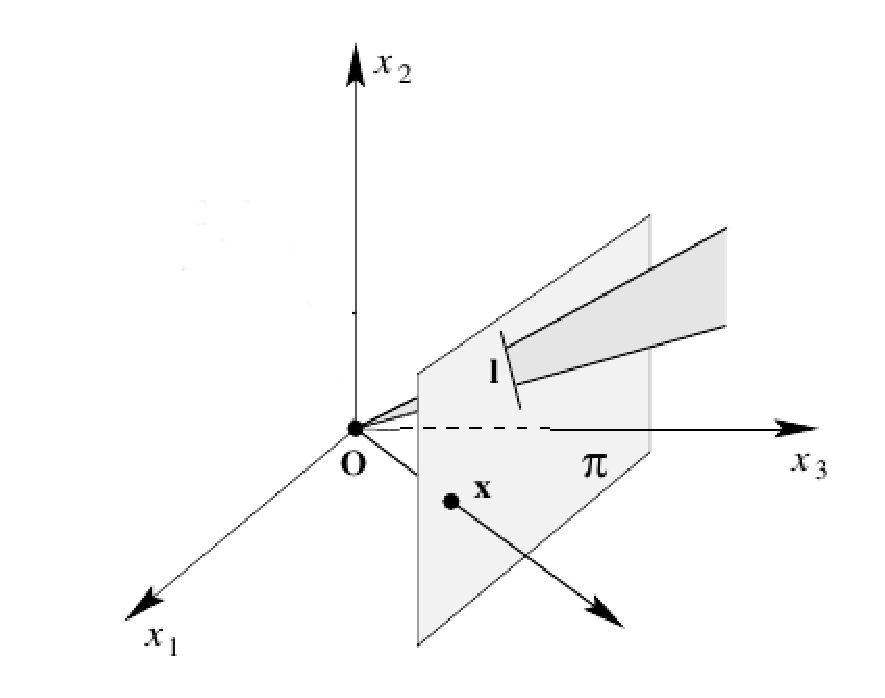
\includegraphics[scale=0.8]{espaco_P2}
\caption{O plano $\pi$ representa o espaço projetivo $\mathbb{P}^2$. Pontos e retas pertencentes a esse espaço são representados, respectivamente, por raios e planos que passam pela origem do $\mathbb{R}^3$.}
\label{plano_P2}
\end{figure}

Podemos pensar no esapaço projetivo como um conjunto de raios passando pela origem do $\mathbb{R}^3$, onde cada raio representa um único ponto, que é a interseção desse raio com o plano $\mathbb{P}^2$. Desta mesma forma, retas em $\mathbb{P}^2$ são formadas por planos. Na figura \ref{plano_P2}, podemos observar com a interseção do raio com o plano define um ponto, assim como a interseção de dois planos definem uma reta.
\\

$\Longrightarrow$ A Cônica


Em geometria Euclidiana, as cônicas são de três tipos principais: elipse, hipérbole e parábola. São definidas, algebricamente, por uma equação do segundo grau em duas variáveis, considerando coordenadas não homogêneas:

\begin{equation*}
a\,x^2+b\,x\,y+c\,y^2+d\,x+e\,y+f=0.
\end{equation*}

Sabemos que um ponto pertence à cônica se ele é solução da equação acima, a qual pode ser representada utilizando multiplicação matricial e vetores em coordenadas homogêneas, com a terceira coordenada configurada como 1:

\begin{center}
$
\begin{array}{cccc}
  (x,y,1)^T 
& \begin{bmatrix}
a & b/2 & d/2\\
b/2 & c & e/2\\
d/2 & e/2 & f
\end{bmatrix}
& \begin{pmatrix}
x\\
y\\
1
\end{pmatrix}
& = 0.
\end{array}
$
\end{center}

Podemos generalizar essas coordenadas homogêneas fazendo as substituições $x = x_{1}/x_{3}$ e $y = x_{2}/x_{3}$, e nossa equação do elípse fica:

\begin{equation*}
a\,x_1^2+b\,x_1\,x_2+c\,x_2^2+d\,x_1\,x_3+e\,x_2\,x_3+f\,x_3^2=0.
\end{equation*}

Novamente em notação matricial:

\begin{center}
$
\begin{array}{cccccc}
  (x_1,x_2,x_3)^T 
& \begin{bmatrix}
  a & b/2 & d/2\\
  b/2 & c & e/2\\
  d/2 & e/2 & f
  \end{bmatrix}
& \begin{pmatrix}
  x_1\\
  x_2\\
  x_3
  \end{pmatrix}
& = 0
& \qquad \text{ou} \qquad
& \x^T\,C\,\x = 0.
\end{array}
$
\end{center}

Já que um ponto pertence à cônica se, e somente se, satisfaz a última equação, temos que $C$ fica definida como a matriz que representa uma cônica no espaço projetivo $\mathbb{P}^2$.

\begin{center}
$
\begin{array}{cc}
C = & \begin{bmatrix}
      a & b/2 & d/2\\
      b/2 & c & e/2\\
      d/2 & e/2 & f
      \end{bmatrix}.
\end{array}
$
\end{center}




\subsubsection{O Espaço Projetivo em Três Dimensões}


$\Longrightarrow$ O Ponto


Analogamente à representação de um ponto no espaço $\mathbb{P}^2$, um ponto no espaço $\mathbb{P}^3$ é repesentado através de coordenadas homogêneas, acrescentando-se uma quarta coordenada ao vetor que representa esse ponto. Desta forma, $\X = (X_1,X_2,X_3,X_4)^T$ e $X_4 \ne 0$, onde $\X$ é a representação em coordenadas homogêneas do ponto $(X,Y,Z)^T \in \mathbb{R}^3$. Para realizar essa mudança basta tomar 

\begin{equation*}
X=X_1/X_4 \,\, ,\, Y=X_2/X_4 \,\,\, \text{e} \,\,\, Z=X_3/X_4.
\end{equation*}


$\Longrightarrow$ O Plano

Temos que a representação algébrica de um plano $\bpi$ no espaço $\mathbb{R}^3$ é dada pela equação

\begin{equation*}
\pi_1\,X+\pi_2\,Y+\pi_3\,Z+\pi_4=0.
\end{equation*}


\subsection{Notação Usada por Fabbri}
Usar figura do artigo.

\subsection{Resumo dos Resultados Fabbri}
Projeção e reconstrução 3D com o uso de tangentes.

%\section{Pesquisas Anteriores para a Determinação de Pose}
 
 O problema da determinação da pose de uma câmera  tem sido estudado extensivamente pela comunidade da área de visão computacional. Vamos citar alguns exemplos da determinação da pose de uma câmera.

\subsection{Usando três Pontos}
O caso mínimo da determinação de uma pose usando três pontos foi estudado por \cite{fischler}, e em seus estudos foi relatado o seguinte problema: 

``Dado um grupo de $m$ pontos de referência, cujas coordenadas 3D são conhecidas em um certo sistema de coordenadas, e dada uma imagem de um subconjunto desses $ m $ pontos de referência, determinar a localização (no sistema de coordenadas desses pontos de referência) do ponto onde a imagem foi registrada."

Assume-se que se conhece a correspondência entre os pontos de referência e os respectivos pontos na imagem, são conhecidos o ponto principal e o comprimento da distância focal para facilitar o cálculo dos ângulos entre pontos de referência a partir do centro da câmera, e por fim, assume-se que a câmera está localizada fora e ``acima" da região convexa formada pelos pontos de referência.
Desta forma, calculando as três distância entre o centro da câmera e  três pontos de referência (chamadas de ``pernas"), é possível determinar a posição da câmera bem como a orientação do plano da imagem. Nota-se que esses três pontos de referência formam um triângulo e, juntamente com o  centro da câmera, forma-se um tetraedro. Para calcular essas três ``pernas" pode-se aplicar a lei dos cossenos e formar um sistema com três equações. Em seguida, [10] explicita uma solução algébrica para o sistema bem como uma solução iterativa, calcula o centro da câmera e a orientação do plano da imagem.

Muitas outras formulações para problemas desse tipo foram comparadas e revisadas por \cite{haralick}. 

\subsection{Usando três Linhas}
 Para correspondência usando linha foi encontrada uma solução mínima usando três linhas e suas correspondências por \cite{chen}, como se segue:

Neste artigo não é determinada a pose de uma câmera, mas sim feita uma exposição para detrminação da localização de objetos em geral, com relação a um detrminiado sistema de coordendas. Sendo $\mathbf{m_i} $ a direção de uma linha $\mathbf{L_i} $ e $\mathbf{n_i} $ o vetor unitário normal a um plano $\mathbf{F_i} $. Além disso, $\mathbf{p_i} $ é a posição de um ponto na linha $\mathbf{L_i} $ e $\mathbf{d_i} $ é a distância entre $\mathbf{F_i} $ e a origem do sistema de coordenadas. O problema pode ser matematicamente formulado:
Dados $\mathbf{m_i} $,$\mathbf{n_i} $,$\mathbf{p_i} $,$\mathbf{d_i} $, determinar $ R $ e $ \mathbf{t} $ de maneira que 
\begin{equation*}
{\bf n}_i^{T}\,R\,{\bf m}_i = 0 \qquad {\bf n}_i^T\,(R\,{\bf p}_i+{\bf t}) = {\bf d}_i
\end{equation*}

As equações significam que, para uma matriz de rotação, o vetor linha rotacionado é perpendicular ao vetor normal. E, para um vetor de translação, o ponto transladado perntencerá ao plano. Mais ainda, toda a linha que contém esse ponto estará contida no plano. Como são necessárias seis restrições para a matriz de rotação e o vetor de translação, precisa-se de pelo menos três pares de correspondência para resolver o problema, pois cada par nos fornece duas equações.

A solução dada por \cite{chen} é chamada solução canônica e consiste basicamente em calcular a matriz de rotação usando a primeira relação, definindo essa matriz com uma multiplicação de outras três matriz de rotação, onde cada uma produz uma rotação em torno de um eixo, os quais formam entre si uma base perpendicular. A primeira relação gera um sistema com duas equações onde é dada uma solução numérica. As entradas do vetor de translação são lineares na segunda relação, e são calculadas após o cálculo da matriz de rotação, usando um sistema com três equações.

Outro desenvolvimento envolvendo linhas pode ser encontrado em \cite{dhome}.

\subsection{Usando Combinação de Pontos e Linhas}
Recentemente, um caso mínimo usando combinação de pontos e linhas foi publicado \cite{ramalingam}. Na correspondência entre pontos, usa-se o fato de que os pontos  ${\bf X}$ 3D na cena, ${\bf x}$ 2D na imagem e ${\bf C}$ o centro da câmera, estão alinhados. Esses pontos são empilhados numa matriz $3\times4$, onde cada submatriz $3\times3$ terá determinante zero por conta da linearidade dos pontos. As entradas do ponto 2D imagem nessa matriz são colocadas em função da matriz de rotação $R$ e do vetor de translação ${\bf t}$, retirados da equação de projeção $\lambda\,{\bf x}={\bf P}\,{\bf X}$.

\begin{center}
$\begin{bmatrix}
C_1 & X_1 & R_{1,1}\,X_1\,+\,R_{1,2}\,X_2\,+\,R_{1,3}\,X_3\,+\,t_1 \\ 
C_2 & X_2 & R_{2,1}\,X_1\,+\,R_{2,2}\,X_2\,+\,R_{2,3}\,X_3\,+\,t_2 \\ 
C_3 & X_3 & R_{3,1}\,X_1\,+\,R_{3,2}\,X_2\,+\,R_{3,3}\,X_3\,+\,t_3 \\ 
1 & 1 & 1
\end{bmatrix} $
\end{center}

Apesar do cálculo de quatro derterminantes na matriz acima, temos apenas duas restrições já que nem todas as equações são L.I.

Uma abordagem similar é construída para as correspondências entre linhas. Uma linha na cena possui pontos extremos ${\bf X}_1$ e ${\bf X}_2$, a linha correspondente na imagem possui extremos ${\bf x}_1$ e ${\bf x}_2$. Esses quatro pontos saõ coplanares juntamente com o centro ${\bf C}$ da câmera e, por isso, o determinante da matriz abaixo deve ser zero.

\begin{center}
$\begin{bmatrix}
C_x & X_{1,x} & X_{2,x} & R_{1,1}\,X_{1,x}\,+\,R_{1,2}\,X_{1,y}\,+\,R_{1,3}\,X_{1,z}\,+\,t_1 \\ 
C_y & X_{1,y} & X_{2,y} & R_{2,1}\,X_{2,x}\,+\,R_{2,2}\,X_{2,y}\,+\,R_{2,3}\,X_{2,z}\,+\,t_2 \\ 
C_z & X_{1,z} & X_{2,z} & R_{3,1}\,X_{3,x}\,+\,R_{3,2}\,X_{3,y}\,+\,R_{3,3}\,X_{3,z}\,+\,t_3 \\ 
1 & 1 & 1 & 1
\end{bmatrix} $
\end{center}

O determinante dessa matriz fornece uma restrição usando a imagem ${\bf x}_1$, mas consegue-se outra restrição com o determinante de uma matriz similar usando a imagem ${\bf x}_2$. Assim, combinando duas linhas e um ponto ou dois pontos e uma linha, obtém-se as seis restrições necessárias. Com uma mudança de coordenadas que satisfaz algumas condições, ficam determinados os pontos na imagem, na cena e o centro da câmera. Além disso, o sistema de equações fica reduzido a um polinômino de grau 4 a 8, bem menor que o original (antes da mudança de coordenadas) que era 64. Outro estudo bastante interessante usando combinações de pontos, linhas e tagentes  pode ser encontrado em \cite{bib:kuang}. Nesse estudo, observa-se ainda a aplicação de técnicas recentes de resolução de sistemas de equações polinomiais multivariadas, baseadas em geometria algébrica. 

\subsection{Usando quatro Pontos não Coplanares}
A generalização para casos não planares, o caso mínimo usando quatro pontos 2D-3D foi primeiramente resolvido por \cite{triggs}. A ideia basica é determinar a pose e a distancia focal usando quatro correspondencias e tomando a matriz de calibraçao com os valores padronizados:

\begin{center}
$\begin{array}{cc}
K =  & \begin{bmatrix}
 0 & 0 & 0 \\ 
 0 & 1 & 0 \\ 
 0 & 0 & 1/f
\end{bmatrix} 
\end{array}$
\end{center}

O primeiro passo é parecido com o algoritmo DLT onde dado um ponto 3D e sua imagem $\lambda\,{\bf x} = P\,{\bf X}$, elimina-se a profundidade $\lambda$ com o produto cruzado ${\bf x}\times P\,{\bf X} = {\bf 0}$ e escolhe-se duas restrições em $P$. Transformando ${\bf x}$ numa matriz de \textit{Householder}, as restrições podem ser reunidas numa matriz $2\,n\times 12$, e no caso do uso de quatro pontos teremos uma matriz $8\times 12$ que tem posto $8$ e deixa $4$ espaços nulos. $P$ pode ser descrita como:

\begin{center}
$P = P(\mu)\equiv\sum_{i=1}^d{\mu_i\,P_i} $,
\end{center}

onde $P_i$ são as matrizes $3\times 4$ correspondentes a cada vetor base do espaço nulo, os quais são calculados numericamente através da decomposição SVD.

Sendo a decomposição $P\simeq K\,R(I| -{\bf t})$, a matriz quádrica absoluta e sua imagem

\begin{center}$
\begin{array}{cc}
\begin{array}{cc}
\Omega \equiv  & \begin{bmatrix}
1 & 0 & 0 & 0 \\ 
0 & 1 & 0 & 0 \\ 
0 & 0 & 1 & 0 \\ 
0 & 0 & 0 & 0
\end{bmatrix} 
\end{array} 
 & \text{e} \quad \omega \equiv P\,\Omega P^{T} \simeq KK^{T} \text{, respectivamente.}
\end{array}$ 
\end{center}

Assim pode-se converter as restrições em $K$ naquelas das candidatas $P(\mu)$ ou nas imagens $\omega$:

\begin{center}
$\omega  = \omega (\mu) \equiv P(\mu)\,\Omega P(\mu)^T$
\end{center}  

Como $K = diag((f,f,1)$ então $K\,K^T = diag(f^2,f^2,1)$ e, consequentemente, 
\begin{center}
$\omega _{1,1} = \omega_{2,2}$ \quad e \quad $\omega_{1,2} = \omega_{1,3} = \omega_{2,3} = 0$
\end{center}

Assim temos um sistema de equações quadráticas nas quatro variáveis $\mu_i$ que tem pelo menos uma solução. Pode-se usar a decomposição SVD para obter os $\mu_i$, sustituí-los em $P(\mu)$ para obter $P$, em seguida fazer a decomposição de $P$ para obter pose e calibração. A matriz resultante é grande, $80\times 56$ mas ainda sim é tratável.


 Outros autores como \cite{bujnak} resoveram para um caso mínimo de quatro pontos para câmeras sem conheciemnto da distância focal e distorção radial.

\subsection{Usando Pontos-Tangentes}
Em \cite{Fabbri:Giblin:Kimia:ECCV12} uma solução é dada usando um problema mínimo de dois pontos-tangentes,$\lbrace ({\bf X}_1^w,{\bf T}_1^w),({\bf X}_2^w,{\bf T}_2^w)\rbrace$, e suas respectivas imagens $\lbrace ({\bf x}_1,{\bf t}_1),({\bf x}_2,{\bf t}_2)\rbrace$. No artigo é demonstrado que a solução pode ser obtida resolvendo um sistema com duas equações:

\begin{center}
$\begin{cases}
{\bf x}_1^T\,{\bf x}_1\,\rho_1^2 - 2\,{\bf x}_1^T\,{\bf x}_2\,\rho_1\,\rho_2 + {\bf x}_2^T\,{\bf x}_2\,\rho_2^2 = ||{\bf X}_1^w - {\bf X}_2^w||\\
Q(\rho_1,\rho_2) = 0,
\end{cases}$
\end{center}

onde $\rho$ é a profundidade em ${\bf x} = \rho\,{\bf X}$, $Q$ é um polinômio de grau 8, e a pose da câmera $R, {\bf \tau}$ relativa ao sistema de coordenadas do mundo é definida por ${\bf X} = R\,{\bf X}^w  + \tau$. 

Fazendo-se umas substituições e isolando $R\, \text{e}\, \tau$ temos:

\begin{center}
$\begin{cases}
R = [({\bf X}_1^w - {\bf X}_2^w)\,{\bf T}_1^w\,{\bf T}_2^w]^{-1} \cdot [\rho_1\,{\bf x}_1 - \rho_2\,{\bf x}_2\,\rho_1\,\frac{g_1}{G_1}\,{\bf t}_1 + \frac{\rho_1'}{G_1}\,{\bf x}_1\,\rho_2\,\frac{g_2}{G_2}\,{\bf t}_2 + \frac{\rho_2'}{G_2}\,{\bf x_2}]\\
\tau = \rho_1\,{\bf x}_1 - R\,{\bf X}_1^w.
\end{cases}$
\end{center}

Em material suplementar estão disponíveis expressões para $\frac{g_1}{G_1}, \frac{g_2}{G_2}\text{(razão das velocidades)}, \rho_1 \,\text{e}\, \rho_2$. 

\texttt{ correspondência necessária é reduzida a uma única correspondência local feita por [20 - koser,koch].Contudo, esta última configuração é muito sensível aos ruídos medidos na correspondência. Para determinação de pose de câmera sem conhecimento da distância focal, o caso com imagens no mesmo plano foi formulado por [1 - abidi,chandra].  Soluções eficientes  e numericamente estáveis foram desenvolvidas por [4 - bujnak et.al.]. Combinando correspondências 2D-2D e 2D-3D, [19 - josephson, astrom, et. al.] investigaram muitos casos mínimos para determinação da pose sem conhecimento da distância focal.   }


%\section{Geometria Trifocal}

\subsection{O Problema}

\subsection{Abordagem por Tensor Trifocal}

\subsection{Abordagem do Nistér}
%\section{Tensor Trifocal: detalhamento da abordagem de Nistér e Schaffalitzky.}

Para abordar um problema trifocal, primeiro \cite{2503343} desenvolvem uma abordagem num sistema bifocal para determinação da rotação e da translação (supondo qua a calibração já seja conhecida) da segunda câmera em relação à primeira, considerando duas imagens de quatro pontos em 3D. Eles demonstram que os epipolos de cada imagem estão restritos a se alojarem numa curva de grau 10, a chamada curva décica, bem como desenvolvem um método para a obtenção dessa curva. De posse dos epipolos, definem a geometria epipolar, resgatam a segunda câmera em relação à primeira e fazem a reconstrução 3D. Com os pontos em 3D e a terceira imagem, resgatam a terceira câmera em relação à primeira. Utilizam essa teoria para desenvolver o que chamaram de solução mais eficiente para época (2006), o notório desafio de estabelecer as poses das câmeras num sistema com três imagens. Vamos incluir os detalhes mais importantes na reprodução desse artigo. 

\begin{figure}[!htb]
\centering
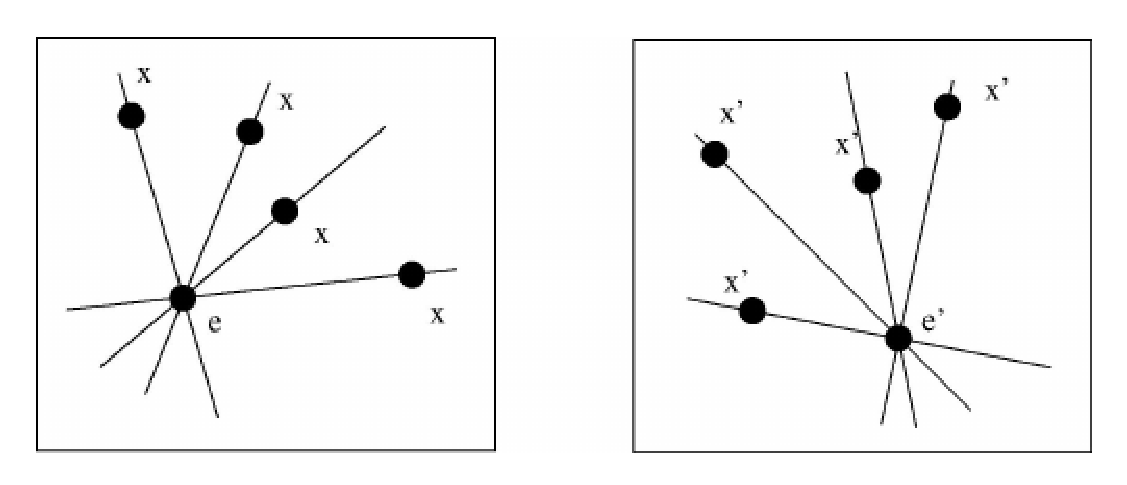
\includegraphics[scale=.85]{retas-epipolares}
\caption{\textit{Feixe de retas passando pelo epipolo em cada imagem, relacionadas duas a duas por uma homografia.}}
\label{retas-epipolares}
\end{figure}

\subsection{O teorema 1.} 

Uma das primeiras afirmações importantes do artigo é de as retas epipolares numa imagem estão homograficamente relacionadas com as retas epipolares na segunda imagem. Dados $n$ correspondências de pontos em duas imagens, a \textit{restrição epipolar} \citep{faugeras93three} pode ser expressa como: os parâmetros projetivos das $n$ retas ligando o epipolo ${\bf e}$ aos pontos ${\bf x}_i$ na primeira imagem, estão homograficamente relacionados com os parâmetros projetivos das $n$ retas ligando o epipolo ${\bf e'}$ aos pontos ${\bf x'}_i$ na segunda imagem. Ou seja, temos uma homografia 1D que relaciona o feixe de retas através ${\bf e}$ com o feixe de retas através ${\bf e'}$ chamada \textit{homografia da reta epipolar}. Podemos visualizar essa situação na figura \ref{retas-epipolares}.


\subsubsection{Detalhamento: a homografia da reta epipolar.} 


Supondo os epipolos na origem do plano de cada imagem, com as retas epipolares passando pelo epipolo, cada reta pode ser parametrizada através do ângulo que ela forma com o eixo das abscissas, denominados $\alpha_1$ e $\alpha_2$ na primeira e segunda imagens respectivamente.
A homografia da reta epipolar pode ser representada pela equação de uma hipérbole alinhada aos eixos perpendiculares, conforme descrito em \cite{Fabbri:Kimia:IJCV2015}.

\begin{equation}\label{eq.hiperbole}
a\,x\,y+b\,x+c\,y+d=0 \qquad \text{ou} \qquad y=\frac{-b\,x-d}{a\,x+c},
\end{equation} 
onde $x=tan\,\alpha_1$ e $y=tan\,\alpha_2$. 

Vemos na figura \ref{fig.reta-epipolar} que cada reta epipolar fica definida por um ponto no eixo da tangente, $(1,tan\,\alpha_1)$ na primeira imagem e $(1,tan\,\alpha_2)$ na segunda, onde consideramos o círculo trigonométrico de raio $1$. Usando esses pontos, a equação da hipérbole pode ser escrita na forma

\begin{equation}\label{eq.homo-reta-epi}
(1\,,\,tan\,\alpha_1)
\overbrace{
\begin{bmatrix}
d&c\\
b&a
\end{bmatrix}
}^{H}
\begin{pmatrix}
1\\
tan\,\alpha_2
\end{pmatrix}
=0,
\end{equation}
sendo 
$\begin{bmatrix}d&c\\b&a\end{bmatrix}$ a homografia procurada.

O problema é que a equação \ref{eq.homo-reta-epi} não está definida para retas epipolares verticais, pois utilizamos a tangente, e uma saída é parametrizar cada reta através da própria definição de tangente, pois assim temos uma representação isotrópica \footnote{É o que se diz de um corpo que, em todas as direções, apresenta as mesmas propriedades ópticas.} para as retas:

\begin{equation}\label{eq.tan.alpha1-2}
x=tan\,\alpha_1=\frac{sen\,\alpha_1 }{cos\,\alpha_1} \qquad \text{e} \qquad y=tan\,\alpha_2=\frac{sen\,\alpha_2}{cos\,\alpha_2}.
\end{equation} 

Desta forma, substituindo \ref{eq.tan.alpha1-2} em \ref{eq.hiperbole} e multiplicando por $cos\,\alpha_1\,cos\,\alpha_2$ temos

\begin{equation*}
a\,sen\,\alpha_1\,sen\,\alpha_2+b\,sen\,\alpha_1\,cos\,\alpha_2+c\,cos\,\alpha_1\,sen\,\alpha_2+d\,cos\,\alpha_1\,cos\,\alpha_2=0.
\end{equation*}

\begin{figure}[!htb]
\centering
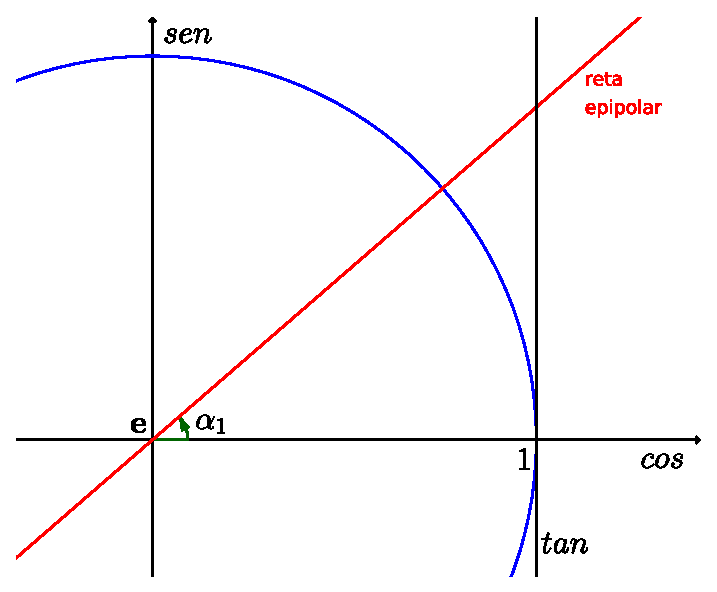
\includegraphics[scale=1]{reta-epipolar-alpha1}
\caption{\textit{Plano da imagem centrado em ${\bf e}$ com a reta epipolar parametrizada por $\alpha_1$.}}
\label{fig.reta-epipolar}
\end{figure}

Com essa conversão, deixamos de parametrizar as retas epipolares pelo eixo da tangente e passamos a parametrizar pelo círculo trigonométrico. Aqui temos um argumento para contagem dos graus de liberdade para fixarmos a relação entre retas epipolares, pois devemos determinar os dois epipolos (duas variáveis cada totalizando quatro graus de liberdade), e mais a matriz que representa a homografia (quatro variáveis mas apenas três graus de liberdade utilizando uma variável para fixar a escala). Portanto, precisamos de no mínimo sete restrições para determinarmos a relação entre duas imagens na geometria epipolar. 

Na nossa abordagem, consideramos o círculo trigonométrico com raio $1$ mas podemos estipular raios arbitrários $r_1$ e $r_2$ em cada uma das imagens que ajuda a garantir estabilidade numérica para a determinação dos coeficientes. Assim, obtemos a equação:

\begin{equation*}
a\,r_1\,sen\,\alpha_1\,r_2\,sen\,\alpha_2+b\,r_1\,sen\,\alpha_1\,r_2\,cos\,\alpha_2+c\,r_1\,cos\,\alpha_1\,r_2\,sen\,\alpha_2+d\,r_1\,cos\,\alpha_1\,r_2\,cos\,\alpha_2=0.
\end{equation*}

Em resumo, as vantagens dessa última representação é ser isotrópica e ter boa estabilidade numérica para escolhas convenientes de $r_1$ e $r_2$, e novamente  na representação matricial:

\begin{equation*}
(r_1\,cos\,\alpha_1\,,\,r_1\,sen\,\alpha_1)
\begin{bmatrix}
d&c\\
b&a
\end{bmatrix}
\begin{pmatrix}
r_2\,cos\,\alpha_2\\
r_2\,sen\,\alpha_2
\end{pmatrix}
=0
\end{equation*}

\subsubsection{Detalhamento: segunda abordagem para mapeamento entre retas epipolares.}\label{sec.homografia-reta-epipolar}


Uma outra forma de pensar sobre essa homografia, encontrada em \cite{Hartley2004}, é considerando que as retas epipolares estão perspectivamente relacionadas com centro em um ponto $Q$ na reta base, conforme a figura \ref{fig.retas-epi-hartley}.

\begin{figure}[!htb]
\centering
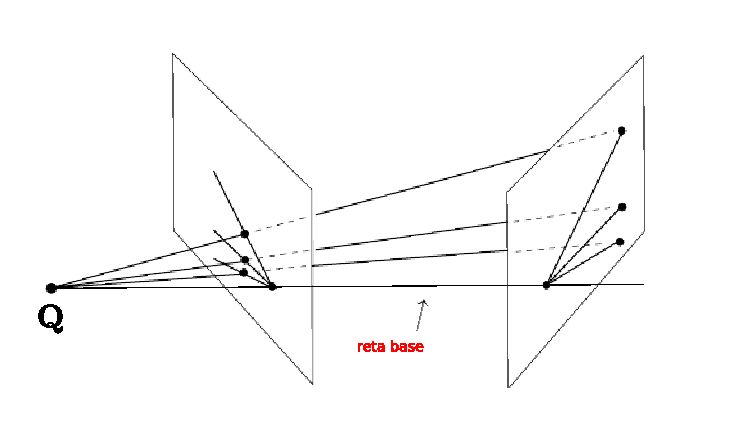
\includegraphics[scale=1]{retas-epipolares-hartley}
\caption{\textit{Retas epipolares com perspectiva centrada em $Q$ na reta base.}}
\label{fig.retas-epi-hartley}
\end{figure}


Suponha que $\lightrgb$ e $\lightrgb'$ sejam duas retas epipolares correspondentes, e ${\bf m}$ é uma reta qualquer que não passa pelo epipolo $\e$. O produto vetorial 

\begin{equation}
{\bf m}\times\lightrgb=\x\qquad\text{ou}\qquad\,[{\bf m}]_\times\,\lightrgb=\x,
\end{equation}
nos fornece o ponto $\x$ de interseção entre essas retas. Pela subseção \ref{sec.matriz-F} temos que

\begin{equation*}
\lightrgb'=F\,\x,
\end{equation*} 
assim, $\lightrgb$ é mapeada a $\lightrgb'$ através da relação 

\begin{equation*}
\lightrgb'=F\,[{\bf m}]_\times\,\lightrgb
\end{equation*}


Uma boa escolha para ${\bf m}$ é a reta $\e$, já que

\begin{equation*}
{\bf m}^\top\e=\e^\top\e\neq0,
\end{equation*}
então $\e$ é uma reta que não passa pelo epipolo $\e$ como desejado. Assim, a homografia da reta epipolar pode ser escrita como 

\begin{equation*}
\lightrgb'=F\,[\e]_\times\,\lightrgb.
\end{equation*}
O argumento é análogo para o mapeamento da segunda imagem para a primeira,

\begin{equation*}
\lightrgb=F^\top [\e']_\times\,\lightrgb'.
\end{equation*}\\

\subsection{Dedução da IAC.}

Uma ferramenta algébrica bastante utilizada nessa abordagem de \citep{2503343} é a imagem da cônica absoluta (IAC em inglês) denotada por ${\bf \omega}$. Como a abordagem assume que as câmeras são calibradas, vamos mostrar que é possível obter a IAC em função da matriz de calibração da câmera $K$.

\subsubsection{Detalhamento: a matriz de calibração, a imagem da cônica absoluta e a imagem da cônica dual absoluta.}

 Inicialmente, vamos determinar a homografia que faz o mapeamento do plano no infinito $\bpi_\infty$ para o plano da imagem na câmera. Se $\X_\infty\in\bpi_\infty$ então pode ser escrito na forma

\begin{equation*}
\X_\infty=({\bf d}^\top,0)^\top
\end{equation*} 
e é projetado por uma câmera geral $P=K\,[R|{\bf t}]$ como

\begin{equation*}
\begin{array}{rcl}
\x&=&P\,\X_\infty\\
&=&K\,[R|{\bf t}]\,({\bf d}^\top,0)^\top\\
&=&K\,R\,{\bf d}.
\end{array}
\end{equation*}
Portanto temos a relação

\begin{equation*}
\x=H\,{\bf d}
\end{equation*}
onde $H=K\,R$. Como a cônica absoluta $\Omega_\infty$ está contida no plano no infinito (contém pontos no infinito), ela pode ser projetada sob a homografia $H$ para computarmos sua imagem.
Sob uma homografia de ponto $\x\rightarrow H\,\x$, uma cônica se transforama de acordo com $C\rightarrow H^{-\top} C\,H^{-1}$, conforme a subseção \ref{sec.trans-proj-H}. De acordo com a subseção \ref{sec.con-absoluta} $C=\Omega_\infty =I$, daí temos

\begin{equation*}
\begin{array}{rcl}
{\bf \omega}&=&H^{-\top}\Omega_\infty\,H^{-1}\\
&=&(K\,R)^{-\top}\,I\,(K\,R)^{-1}\\
&=&K^{-\top}R^{-\top}R^{-1}K^{-1}\\
&=&K^{-\top}K^{-1}
\end{array}
\end{equation*}
pois $R$ é uma matriz de rotação e portanto satisfaz $R^{-\top}R^{-1}=I$. Assim, de posse de uma câmera calibrada é simples obter a IAC.

Analogamente ao que é feito na subseção \ref{sec.conica-dual}, podemos definir a imagem dual da cônica absoluta (sigla DIAC em inglês), denotada por $\omega^*$, a partir de $\omega$ como

\begin{equation*}
\omega^*=\omega^{-1}=K\,K^\top.
\end{equation*}
Esta é uma cônica definida por retas e é a imagem da quádrica dual absoluta ${\tt Q^*_\infty}$, definida na subseção \ref{sec.quadrica-dual-abs}. A imagem é dada por

\begin{equation*}
\omega^*=P\,{\tt Q^*_\infty}P^\top,
\end{equation*}
conforme a subseção \ref{sec.proj-quadricas}.\\

\subsection{O teorema 2.}\label{sec.teorema-2}


Para a correspondência entre retas tangentes às duas cônicas ${\bf \omega}$ e ${\bf \omega'}$ podemos utilizar a restrição \textit{Kruppa}: as duas retas tangentes à ${\bf \omega}$ e passando por $\e$, estão relacionadas por uma homografia de reta epipolar às duas tangentes à ${\bf \omega'}$ passando por $\e'$. Na figura \ref{epipolar-kruppa} podemos observar as restrições epipolar e Kruppa simultaneamente.

\begin{figure}[!htb]
\centering
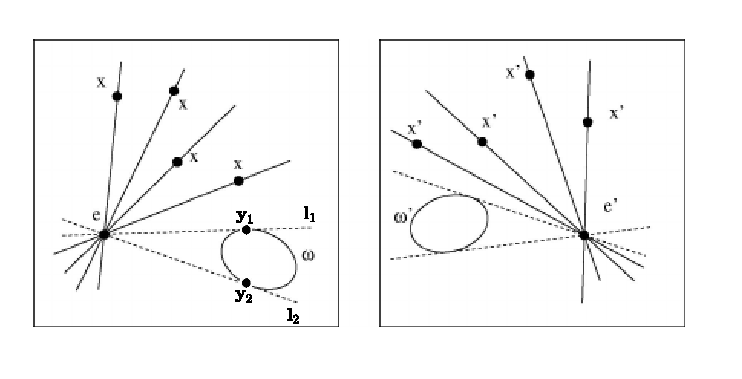
\includegraphics[scale=1.2]{restricao-epipolar-kruppa}
\caption{\textit{Retas epipolares tangentes às cônicas ${\bf \omega}$ e ${\bf \omega'}$.}}
\label{epipolar-kruppa}
\end{figure}

A restrição Kruppa foi originalmente introduzida por \cite{faugeras92} e está relacionada com uma cônica contida num plano no espaco 3D e suas imagens nas câmeras $1$ e $2$, e é válida para cônicas gerais, mas aqui no nosso caso vamos tratar especificamente da cônica absoluta $\Omega_\infty$ contida no plano infinito $\bpi_\infty$ no espaco, e as imagens da cônica absoluta (IAC) ${\bf \omega}$ e ${\bf \omega'}$.


\subsubsection{Detalhamento: as restrições Kruppa.}


 Sendo ${\bf \omega}^*$ e ${{\bf \omega}^*}'$ as respectivas cônicas duais (DIAC), considere um plano passando pelo centro das duas câmeras e tangenciando essa cônica $\Omega_\infty$ no espaco. Por construção, esse plano vai projetar uma reta epipolar em cada imagem onde cada reta será tangente às imagens ${\bf \omega}$ e ${\bf \omega'}$ da cônica $\Omega_\infty$, observado na figura \ref{geometria-kruppa}. E suponha ainda que $\lightrgb_1$ e $\lightrgb_2$ sejam as retas tangentes à cônica ${\bf \omega}$ na primeira imagem conforme a figura \ref{epipolar-kruppa}. Com essas duas retas tangentes podemos construir uma cônica degenerada $D$ (posto $1$ ou $2$) da seguinte maneira:  

\begin{equation}\label{eq.def.con.deg}
D=[\e]_\times\,{\bf \omega}^*\,[\e]_\times \qquad \text{ou, como outra construção} \qquad D=\lightrgb_1\,\lightrgb_2^\top + \lightrgb_2\,\lightrgb_1^\top
\end{equation}

Para mostrar que $D$ é uma cônica (ponto) temos que verificar que é válida a relação $\y_1^\top D\,\y_1=0$, onde $\y_1\in\lightrgb_1$.

\begin{equation*}
\begin{array}{rcll}
\y_1^\top\,D\,\y_1&=&\y_1^\top [\e]_\times\,{\bf \omega}^*\,[\e]_\times\,\y_1&\\
&=&([\e]^\top_\times\,\y_1)^\top {\bf \omega}^*\,[\e]_\times\,\y_1&\\
&=&\lightrgb_1^\top {\bf \omega}^*\,\lightrgb_1& \qquad\text{pois}\qquad\lightrgb_1=\e\times\y_1\\
&=&0&
\end{array}
\end{equation*}
onde a última passagem segue do fato de ${\bf \omega}^*$ ser dual. Observe que usamos $[\e]^\top_\times\,\y_1=[\e]_\times\,\y_1$ quando na verdade $[\e]^\top_\times=-[\e]_\times$, mas aqui a diferença de escala é irrelevante. Analogamente, para a segunda definição de $D$:

\begin{figure}[!htb]
\centering
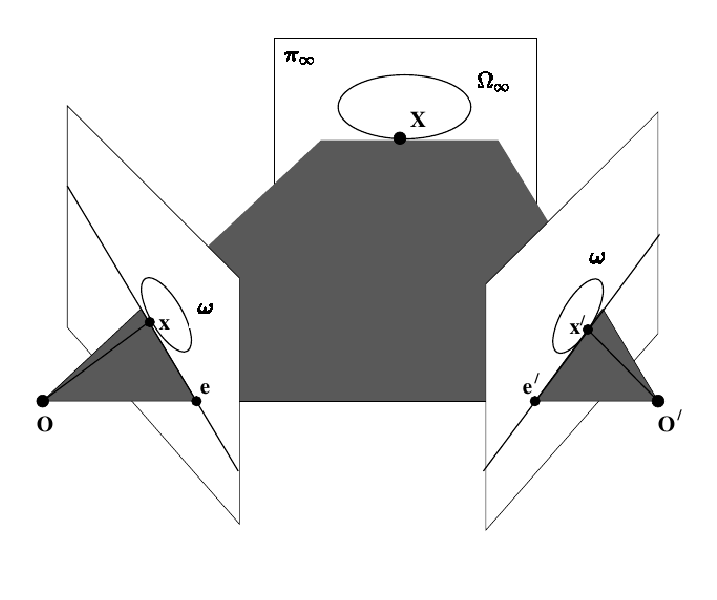
\includegraphics[scale=1.1]{geometria-kruppa}
\caption{\textit{Um plano epipolar tangenciando uma cônica no espaco 3D projeta retas epipolares que tangenciam as cônicas nos planos das imagens}.}
\label{geometria-kruppa}
\end{figure}

\begin{equation*}
\y_1^\top\,D\,\y_1=\y_1^\top \lightrgb_1\,\lightrgb_2^\top + \lightrgb_2\,\lightrgb_1^\top\y_1=0
\end{equation*}
pois como $\y_1\in\lightrgb_1$ então $\y_1^\top \lightrgb_1=\lightrgb_1^\top\y_1=0$. Observamos que o desenvolvimento anterior é análogo para $\lightrgb_2$.

Na segunda imagem, analogamente à primeira, $D'=[\e']_\times\,{{\bf \omega}^*}'\,[\e']_\times$ e se transforma de acordo com a regra $D'=H_\infty^{-\top}D\,H_\infty^{-1}$ na subseção \ref{sec.trans-proj-H}. O símbolo $\infty$ se deve ao fato de que a homografia foi deduzida de maneria similar àquela da subseção  \ref{sec.homografia}, apenas com a diferença de ter sido com base no plano no infinito. Assim:

\begin{equation}\label{eq.kruppa}
\begin{array}{rcll}
[\e']_\times\,{{\bf \omega}^*}'\,[\e']_\times&=&D'&\\
&=&H_\infty^{-\top}D\,H_\infty^{-1}&\\
&=&H_\infty^{-\top}[\e]_\times\,{\bf \omega}^*\,[\e]_\times\,H_\infty^{-1}&\qquad\text{pois}\qquad D=[\e]_\times\,{\bf \omega}^*\,[\e]_\times\\
&=&F\,\omega^* F^\top,&
\end{array}
\end{equation}
onde $F=H_\infty^{-\top}\,[\e]_\times$ conforme a subseção \ref{sec.matriz-F}. 


Da relação \ref{eq.kruppa} são extraídas as duas equações quadráticas independentes eliminando-se o fator de escala, onde tais equações são conhecidas como as restrições de Kruppa. 


\subsection{Mudança de coordenadas projetivas.}

De acordo com \cite{kneebone}, podemos escolher as coordenadas projetivas de forma que os quatro pontos também tenham as mesmas coordenadas em cada imagem. Ou seja, podemos assumir que ${\bf x}_i = {\bf x'}_i$ pensando nos dois planos de imagem como registrados no mesmo sistema de coordenadas. Vejamos como isso pode ser feito.

\subsubsection{Detalhamento: corregistro de pontos pertencentes a diferentes planos de imagem.}\label{sec.corregistro-pontos}
Suponha a existência de pontos em correspondêcia em dois planos de imagem relacionados por uma transformação projetiva $\x'=H\,\x$, onde $\x\in {\mathbb{P}^2}$ e $\x'\in {\mathbb{P'}^2}$. Fazendo as seguintes mudanças de coordenadas projetivas

\begin{equation}\label{eq.igualando-coordenadas}
\begin{array}{rcl}
\overline{\x}\,&=&I\,\x\\
\overline{\x}'&=&H^{-1}\x',
\end{array}
\end{equation}
temos que $\x=\overline{\x}$ e $\x'=H\,\overline{\x}'$. Substituindo essas duas últimas igualdades em $\x'=H\,\x$ temos

\begin{equation*}
\begin{array}{rcll}
\x'&=&H\,\x&\Rightarrow\\
H\,\overline{\x}'&=&H\,\overline{\x}&\Rightarrow\\
\overline{\x}'&=&H^{-1}H\,\overline{\x}&\Rightarrow\\
\overline{\x}'&=&\overline{\x}.&
\end{array}
\end{equation*}
Cabe ressaltar que as mudanças de coordenadas em \ref{eq.igualando-coordenadas} não altera nosso desenvolvimento, já que aqui nos interessa propriedades que são invariantes sob transformações projetivas, como tangências, interseções e raz\~ao cruzada.

\subsection{O teorema 3.}\label{sec.teorema-3}

Aplicando as mudanças de coordenadas descritas na subsec\~ao \ref{sec.corregistro-pontos} nos quatro pontos e nos epipolos, a restrição epipolar pode ser convertida em: os epipolos ${\bf e}$ e ${\bf e'}$ juntamente com os quatros pontos, que obedecem a restrição epipolar, devem estar alojados numa cônica $B$ e, reciprocamente, dois epipolos ${\bf e}$ e ${\bf e'}$ que são concônicos com quatro pontos na imagem satisfazem a restrição epipolar. 

\subsubsection{Detalhamento: argumentação do teorema.}

Pela subseção \ref{sec.definicao-conica}, uma cônica fica determinada por cinco pontos, como temos quatro pontos na imagem vamos deixar a cônica $B$ na dependência de $\e$ (o quinto ponto necessário). Analogamente, o epipolo $\e'$ também define uma cônica com os quatro pontos na imagem, digamos $B'$. Pela subsec\~ao \ref{sec.homografia-reta-epipolar}, existe a homografia da reta epipolar que relaciona essas quatro retas de cada feixe passando por $\e$ e $\e'$. Pelo teorema de Steiner, \citep{kneebone}, se dois feixes de retas passando por $\e$ e $\e'$ estão homograficamente relacionados, o ponto de interseção entre retas correspondentes desses feixes descreve uma cônica que passa por $\e$ e $\e'$. Portanto $B=B'$ e todos os seis pontos em questão são concônicos.


Reciprocamente, pelo teorema de Chasles em \citep{kneebone}, se quatro pontos $\x_i$ numa cônica formam um feixe de retas concorrentes em um quinto ponto $\e\in B$, a razão cruzada entre as quatro retas não depende da posição de $\e$. Assim, a razão cruzada  do feixe concorrente em $\e$ é igual a do feixe concorrente em $\e'$. Pela subseção \ref{sec.geometria-1D}, a razão cruzada num feixe de retas é igual à razão cruzada entre os quatro pontos de interseção de uma reta qualquer com o feixe. Pelo corolário ainda na subseção \ref{sec.geometria-1D}, dois conjuntos de quatro pontos colineares têm a mesma razão cruzada se, e somente se, correspondem sob uma homografia.  


Esta cônica $B=B(\e)$ será bastante importante durante a abordagem pois, se os dois epipolos são concônicos com os quatro pontos na imagem, figura \ref{pontos-conconicos}, existe uma \textit{única} homografia de reta epipolar que faz a relação das quatro retas através ${\bf e}$ com as quatro retas através ${\bf e'}$. 

\begin{figure}[!htb]
\centering
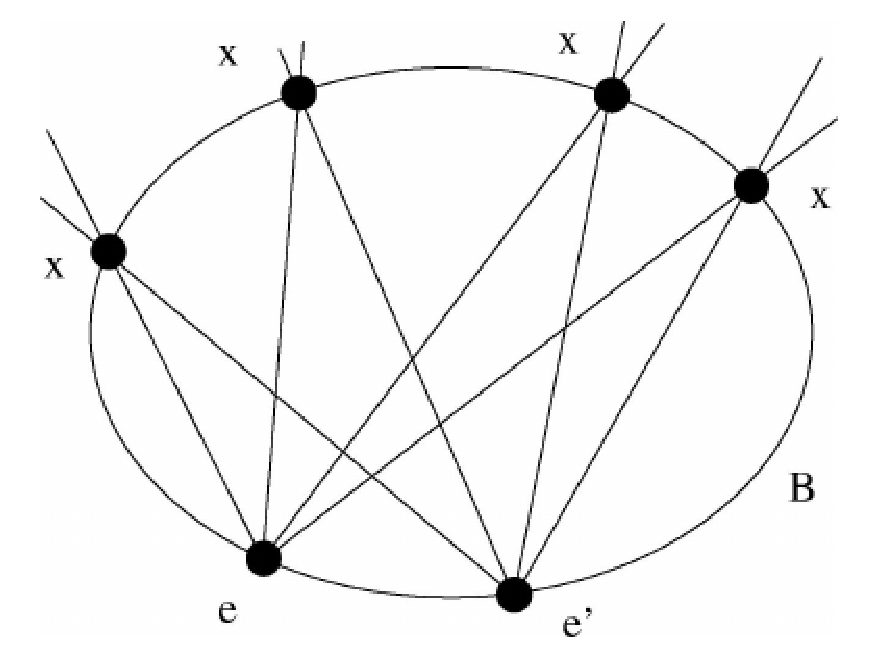
\includegraphics[scale=.85]{pontos-conconicos}
\caption{\textit{Epipolos concônicos com os quatro pontos na imagem produzem homografia única.}}
\label{pontos-conconicos}
\end{figure}

\subsection{O teorema 4.}

Note que podemos parametrizar o feixe de retas passando por ${\bf e'}$ (ou ${\bf e}$) por pontos pertencentes à cônica $B$, pois retas correspondentes nos dois feixes intersectam $B$ no mesmo ponto. Desta forma, o teorema 4 é anunciado como: as restrições de calibração são equivalentes à condição de que as duas retas tangentes à cônica ${\bf \omega}$ e passando por ${\bf e}$, intersectam a cônica $B$ nos mesmos dois pontos adicionais que as retas tangentes à ${\bf \omega'}$ e passando por ${\bf e'}$. 

\subsubsection{Detalhamento: argumentação do teorema.}
Na subseção \ref{sec.teorema-2}, vimos que as duas retas tangentes à conica $\omega$ estão projetivamente relacionadas com as duas tangentes à cônica $\omega'$. Pelo teorema de Steiner, na subseção \ref{sec.teorema-3}, o ponto de interseção entre duas retas correspondentes, em dois feixes homograficamente relacionados, descrevem uma cônica. Assim, as retas tangentes à cônica $\omega$ se intersectam às retas tangentes à cônica $\omega'$ em dois pontos adicionais sobre a cônica $B$. 

Isto é, as projeções de ${\bf \omega}$ e ${\bf \omega'}$ em $B$, através dos respectivos epipolos, devem coincidir. Essa construção geométrica pode ser visualizada na figura \ref{omega-B} e será a fundação para o resto da abordagem. 

\begin{figure}[!htb]
\centering
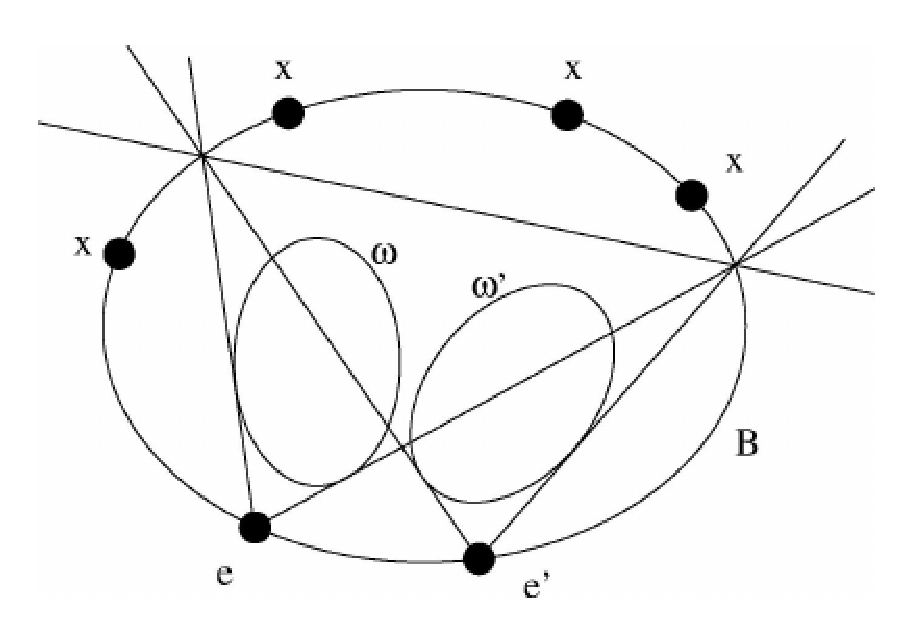
\includegraphics[scale=.85]{projecao-omega-B}
\caption{\textit{Os pontos de interseção das tangentes com a cônica $B$ coincidem, ocasionando a coincidência das projeções das cônicas ${\bf \omega}$ e ${\bf \omega'}$ na cônica $B$.}}
\label{omega-B}
\end{figure}

\subsection{O teorema 5.}

A demonstração desse teorema é dada em \cite{2503343} e vamos incluir alguns detalhes.
Podemos pensar na representação da projeção de  ${\bf \omega}$ e ${\bf \omega'}$ em $B$ como a reta que liga os dois pontos de interseção das tangentes com $B$. Essa reta que liga os dois pontos de interseção, de acordo com a projeção de ${\bf \omega}$ através do epipolo ${\bf e}$ é representada por $({\bf \omega}\diamond B)\,{\bf e}$, e a cônica $({\bf \omega}\diamond B)$ é definida como:

\begin{equation}\label{eq.conica-diamond}
(\omega \diamond B)\equiv 2\,B\,\omega^*B - tr(\omega^*\,B)\,B,
\end{equation}
onde $\omega^*$ é a matriz adjunta de $\omega$.

A equação \ref{eq.conica-diamond} é uma fórmula projetivamente invariante de uma cônica. Para ver isso, basta tomar uma configuração genérica para as cônicas $B$ e $\omega^*$, digamos

\begin{equation*}
B=
\begin{bmatrix}
a&b&c\\
b&d&e\\
c&e&f
\end{bmatrix}
\qquad\text{e}\qquad
\omega^*=
\begin{bmatrix}
g&h&i\\
h&j&l\\
i&l&m
\end{bmatrix},
\end{equation*} 
e efetuar as multiplicações constantes na equação \ref{eq.conica-diamond}. Lembrando que o traço de uma matriz é definido pela soma dos elementos da diagonal principal, o resultado das multiplicações é uma matriz simétrica, que pela subseção \ref{sec.definicao-conica}, representa uma cônica. Pela subseção \ref{sec.trans-proj-H}, uma homografia leva uma cônica em outra cônica, a qual mantém as características invariantes sob transformação projetiva.

\subsubsection{Representação canônica de uma cônica.}

Como vimos na subseção \ref{sec.espaco-P2}, o plano projetivo $\mathbb{P}^2$ tem seus pontos representados por vetores homogêneos com três componentes. Da algebra linear sabemos que o espaço $\mathbb{R}^3$ também tem seus pontos representados por vetores com três componentes. Portanto, existe uma analogia entre as representações mesmo que no plano projetivo a relação entre vetores e pontos não seja biunívoca como em $\mathbb{R}^3$. Da mesma forma que podemos escolher a base canônica para representar vetores em $\mathbb{R}^3$, fazendo a devida transformação projetiva do sistema de coordeandas, podemos escolher uma base para representação do plano projetivo incluindo um \textit{vetor unitário} ${\bf u}=(1,1,1)$. Assim, cada ponto em $\mathbb{P}^2$ pode ser representado em termos da base \{$\x_1=(1,0,0),\x_2=(0,1,0),\x_3=(0,0,1),{\bf u}=(1,1,1)$\} onde os três primeiros vetores são chamados {\it pontos de referência}. Para detalhes ver \citep{kneebone}.

Os pontos de referência, que são linearmente independentes, formam os vértices de um triângulo chamado \textit{triângulo de referência}, com o ponto unitário no interior do triângulo. Esse triângulo vai servir como uma base para a representação do plano projetivo, conforme a figura \ref{fig.triangulo-referencia}. Por exemplo, representando um ponto qualquer por $\x=(x,y,z)^\top$ e uma reta qualquer por $\lightrgb=(a,b,c)^\top$ a reta determinada pelos pontos $\x_1$ e ${\bf u}$ tem equação $z-y=0$.

\begin{figure}[!htb]
\centering
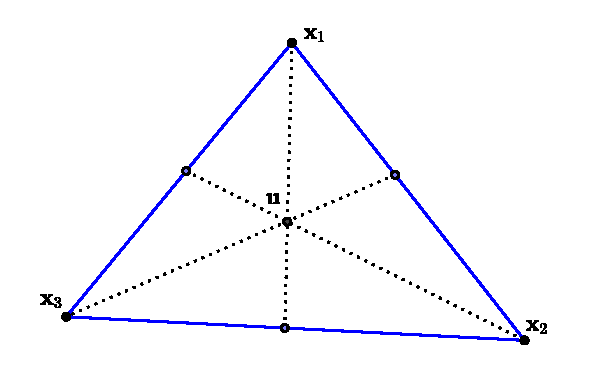
\includegraphics[scale=1]{triangulo-referencia}
\caption{{\it Triângulo de referência com vértices determinados por três vetores que, juntamente com o vetor unitário, servem de base para representação do plano projetivo.}}
\label{fig.triangulo-referencia}
\end{figure}

Pois, se $\x_1\in\lightrgb$ e ${\bf v}\in\lightrgb$ então

\begin{equation}\label{eq.exemplo-tri-referencia}
\lightrgb^\top{\bf u}=0\Rightarrow a+b+c=0\qquad\text{e}\qquad\lightrgb^\top\x_1=0\Rightarrow a=0.\qquad\text{Assim,}\quad c=-b.
\end{equation}

Dado um ponto qualquer $\x\in\lightrgb$ a equação da reta fica

\begin{equation*}
\lightrgb^\top\x=0\Rightarrow a\,x+b\,y+c\,z=0,
\end{equation*}
usando \ref{eq.exemplo-tri-referencia} temos que

\begin{equation*}
-c\,y+c\,z=0\Rightarrow z-y=0,
\end{equation*}
já que $c=0$ pois do contrário $\lightrgb$ representaria um ponto no infinito.

Existem algumas formas padronizadas pelas quais a representação de uma cônica $C$ pode ser simplificada através da escolha conveniente de uma estrutura de referência. Umas dessas escolhas é tomar o triângulo de referência como tendo dois de seus lados tangentes à cônica, e o terceiro lado como reta polar em relação ao vértice oposto, e escolher um ponto  da cônica como ponto unitário. Ver figura \ref{fig.conica-tri-referencia}.

\begin{figure}[!htb]
\centering
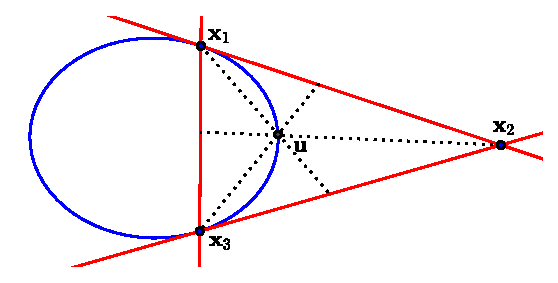
\includegraphics[scale=1]{conica-tri-referencia}
\caption{{\it Uma cônica $C$ numa relação polo-polar com um triângulo de referência que representa o plano projetivo $\mathbb{P}^2$}.}
\label{fig.conica-tri-referencia}
\end{figure}

Como vimos na subseção \ref{sec.definicao-conica}, uma cônica $C$ pode ser representada na forma matricial com coordenadas homogêneas como

\begin{equation*}
\begin{pmatrix}
x&y&z
\end{pmatrix}
\begin{bmatrix}
a&b/2&c/2\\
b/2&d&e/2\\
c/2&e/2&f
\end{bmatrix}
\begin{pmatrix}
x\\
y\\
z
\end{pmatrix}
=0
\end{equation*}
ou através da equação

\begin{equation*}
a\,x^2+b\,x\,y+d\,y^2+c\,x\,z+e\,y\,z+f\,z^2=0.
\end{equation*}

Supondo que a cônica passe pelos pontos $\x_1=(1,0,0)^\top$ e $\x_3=(0,0,1)^\top$ temos que

\begin{equation*}
\x_1\in C\Rightarrow a=0\quad\text{e}\quad\x_3\in C\Rightarrow f=0,
\end{equation*}
daí a equação da cônica será 

\begin{equation}\label{eq.reducao-parcial-conica}
d\,y^2+b\,x\,y+c\,x\,z+e\,y\,z=0.
\end{equation}

Consirede a reta $\lightrgb=(l_1,l_2,l_3)^\top$ que passa pelos pontos $\x_1$ e $\x_3$,

\begin{equation*}
\lightrgb^\top\x_1=
\begin{pmatrix}
l_1&l_2&l_3
\end{pmatrix}
\begin{pmatrix}
1\\
0\\
0
\end{pmatrix}
=0
\Rightarrow l_1=0,
\end{equation*} 

\begin{equation*}
\lightrgb^\top\x_1=
\begin{pmatrix}
l_1&l_2&l_3
\end{pmatrix}
\begin{pmatrix}
0\\
0\\
1
\end{pmatrix}
=0
\Rightarrow l_3=0,
\end{equation*} 
e portanto $\lightrgb=(0,l_2,0)^\top$.

Observando que $\lightrgb$ está numa relação polo-polar com o ponto $\x_2$, pela subseção \ref{sec.polo-polar} temos que $C\,\x_2=\lightrgb$, daí

\begin{equation*}
\begin{bmatrix}
a&b/2&c/2\\
b/2&d&e/2\\
c/2&e/2&f
\end{bmatrix}
\begin{pmatrix}
0\\
1\\
0
\end{pmatrix}
=
\begin{pmatrix}
b/2\\
d\\
e/2
\end{pmatrix}
=
\begin{pmatrix}
0\\
l_2\\
0
\end{pmatrix},
\end{equation*}
e teremos $b=e=0$ e $d=l_2$.

Assim a equação \ref{eq.reducao-parcial-conica} toma a forma

\begin{equation}\label{eq.reducao-parcial2-conica}
l_2\,y^2+c\,x\,z=0\quad\text{e}\quad y^2=k\,x\,z\quad\text{com}\quad k=\frac{-c}{l_2}.
\end{equation}

A cônica $C$ passa também pelo ponto unitário ${\bf u}=(1,1,1)$, assim substituindo na equação \ref{eq.reducao-parcial2-conica} temos que $k=1$, e a equação da cônica se reduz finalmente a 

\begin{equation}\label{eq.reducao-total-conica}
y^2=x\,z,
\end{equation}
que é a equação conônica da cônica.

\subsubsection{Representação canônica paramétrica.}
A equação \ref{eq.reducao-total-conica} pode ser escrita na forma 

\begin{equation*}
(\frac{y}{z})^2=\frac{x}{z},
\end{equation*}
e fazendo as substituições $\displaystyle{\frac{y}{z}=\theta}$ e $\displaystyle{\frac{x}{z}=\theta^2}$ temos $x:y:z=\theta^2:\theta:1$.
A representação paramétrica de uma cônica própria $(\theta^2,\theta,1)$ é realmente uma parametrização da curva, no sentido de que existe uma relação biunívoca entre cada ponto da curva e o valor do parâmetro. No caso do artigo de \citep{2503343} esta formalização é bastante útil pois, como a cônica $B$ está em função do quinto ponto, o epipolo $\e$, temos que esse ponto, e consequentemente a cônica, pode ser definida apenas pelo parâmetro $\theta$.

 
Note que a reta $(\omega \diamond B)\,{\bf e}$ é a reta polar de ${\bf e}$ com relação à cônica $(\omega \diamond B)$. Está sendo usada a relação polo-polar definida pelo locus da cônica $(\omega \diamond B)$ para executar a projeção. Há uma breve explanação sobre a relação polo-polar na subseção \ref{sec.polo-polar}. Já que os pontos de interseção das tangentes com $B$ são os mesmos para as duas cônicas $\omega$ e $\omega'$, pode ser verificado que, dado que ${\bf e}$ e ${\bf e'}$ são concônicos com quatro pontos na imagem, a restrição Kruppa é equivalente à restrição de que as retas polares $(\omega \diamond B)\,{\bf e}$ e $(\omega' \diamond B)\,{\bf e'}$ coincidem.


Note que $(\omega \diamond B) = B\,(\omega \cdot B)$ se definirmos a homografia

\begin{equation}
(\omega \cdot B) \equiv 2\,\omega^*\,B - tr(\omega^*\,B)\,I,
\end{equation}
onde está sendo ``cancelado" $B$ na definição de $(\omega \diamond B)$. 


Como $(\omega' \diamond B)\,{\bf e}$ e $(\omega' \diamond B)\,{\bf e'}$ coincidem e usando a equivalência anterior, podemos demonstrar que 

\begin{equation}
(\omega' \cdot B)\,{\bf e'} \sim (\omega \cdot B)\,{\bf e}
\end{equation} 
(onde $\sim$ significa igualdade a menos da escala) o que implica num mapeamento de sétimo grau 

\begin{equation}
{\bf e} \rightarrow {\bf e'} \sim (\omega' \cdot B)^*\,(\omega \cdot B)\,{\bf e}.
\label{funcao-de-e}
\end{equation}

No artigo também é domonstrado que a restrição Kruppa disponibiliza quatro soluções (dois pares de soluções coincidentes) para cada ${\bf e}$, e as soluções são as interseções (figura \ref{inter-B-C}) de $B$ com a cônica 

\begin{equation}
C \equiv (\omega \cdot B)^\top\,(\omega' \cdot B)^{*\,\top}\,B\,(\omega' \cdot B)^*(\omega \cdot B).
\end{equation}

\begin{figure}[!htb]
\centering
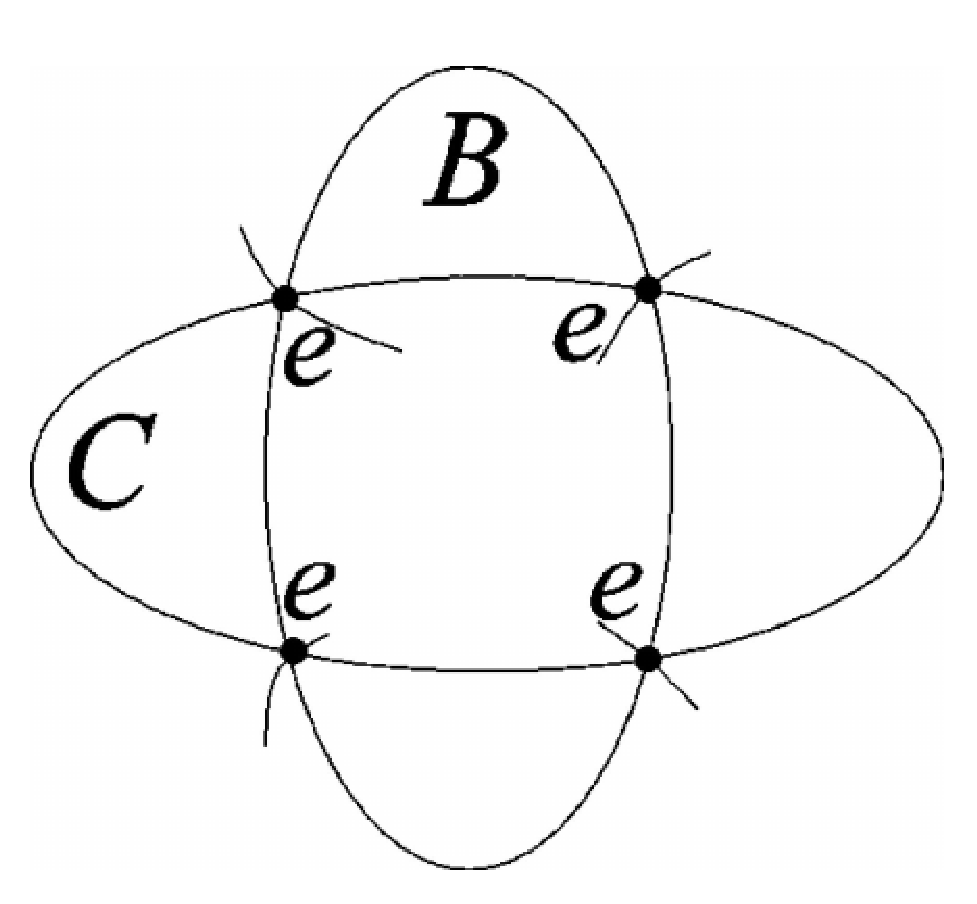
\includegraphics[scale=.6]{intersecao-C-B}
\caption{\textit{Epipolos que satisfazem as restrições de projeção e de calibração podem ser encontrados como as interseções das cônicas B e C.}}
\label{inter-B-C}
\end{figure}

Um epipolo ${\bf e}$ que gera uma cônica $B$ satisfaz à equação de décimo-sexto grau

\begin{equation}
{\bf e}^\top\,C\,{\bf e} = 0
\label{dezesseis}
\end{equation}
se, somente se, ele satisfaz às restrições de projetividade e de calibração. No caso em que a cônica $B$ pode se degenerar em um par de retas, a homografia $(\omega \cdot B)$ permuta as retas do par e assim, a equação \ref{dezesseis} descreve também seis retas passando por cada par dos quatro possíveis epipolos na imagem. Algebricamente, isso significa que a equação \ref{dezesseis} tem $|B|$ como um fator. Na figura \ref{plot-C} podemos observar duas plotagens da curva de dezesseis graus, uma com e outra sem a visualização dessas seis retas.

\begin{figure}[!htb]
\centering
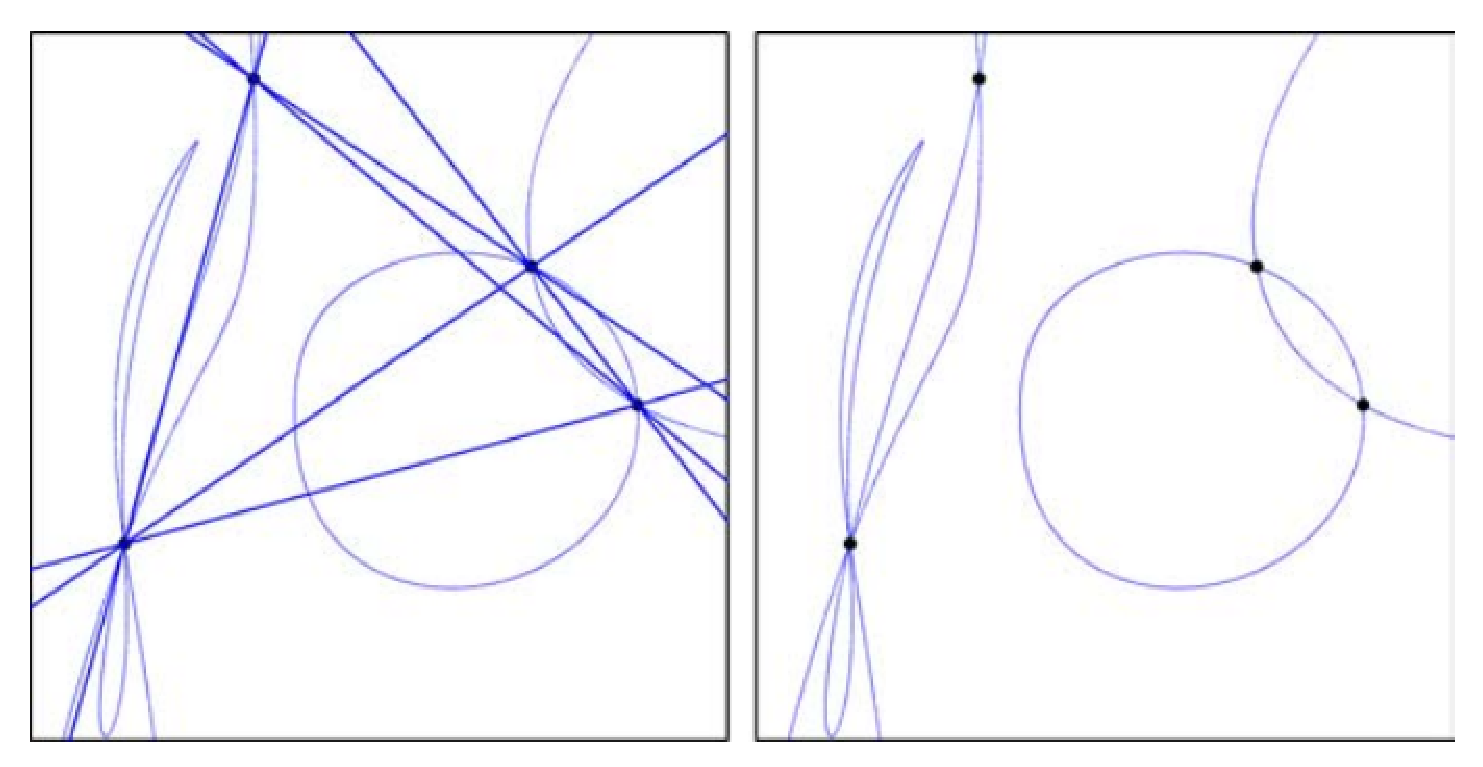
\includegraphics[scale=.6]{plotagem-C}
\caption{\textit{Podemos observar o lugar geométrico dos possíveis epipolos definido pela equação de décimo-sexto grau, a qual define (alem das curvas) as possíveis seis retas. A direita, a mesma imagem sem as retas.}}
\label{plot-C}
\end{figure}

Qualquer epipolo ${\bf e}$ para o qual $|B|\ne0$ satisfaz as restrições de projetividade e calibração se, e somente se, ${\bf e}$ satisfaz a equação de décimo grau remanescente de $e^\top\,C\,e=0$, ou seja, a equação restante após a eliminação do $|B|\ne0$. Geometricamente, temos que os pontos não podem se alojar em quaisquer das seis retas por conta da restrição de calibração. É possível remover $|B|\ne0$ da equação \ref{dezesseis} para se chegar à equação de décimo grau e o trabalho é algebricamente pesado mas também pode ser inteiramente encontrado em \cite{kneebone}. A curva de décimo grau é descrita pela equação

\begin{equation}
e^\top\,G\,e=0,
\label{dez}
\end{equation}
onde 
\begin{equation}
G=4\,U^\top\,D'^*\,B^*\,D'^*\,U-4\,t'^2\,B\,D\,D'^*\,(D\,B-t\,I)+s\,D^*-t^2\,t'^2\,D'^*
\label{conica-G}
\end{equation}
com as definições:

\begin{equation}
\begin{array}{rcl}
D&\equiv&\omega^*,\\
t&\equiv&tr(D\,B),\\
U&\equiv&(\omega \cdot B)\,\,\, \text{e}\\
s&=&(16\,|B|\,|D'|\,t'+t'4-4\,t'2\,tr(B*\,D'*)).
\end{array}
\end{equation}

A partir das consideraçoes feitas até aqui, podemos expor o principal resultado de \cite{kneebone}, o qual afirma que um ponto é um candidato a epipolo de acordo com as restrições de projetividade e calibração se, e somente se, satisfaz a equação de décimo grau definida em \ref{dez}. O que é equivalente ao fato de que ${\bf e}$ deve se alojar na cônica $G$ definida em \ref{camera-G}. Para um epipolo ${\bf e}$ qualquer na curva de décimo grau, o outro epipolo ${\bf e'}$ é calculado pela função de sétimo grau ${\bf e'} \sim U'*\,U\,{\bf e}$, dada em \ref{funcao-de-e}. Na figura \ref{curva-10} observamos alguns exemplos de curvas de décimo grau com seus possíveis epipolos. 

\begin{figure}[!htb]
\centering
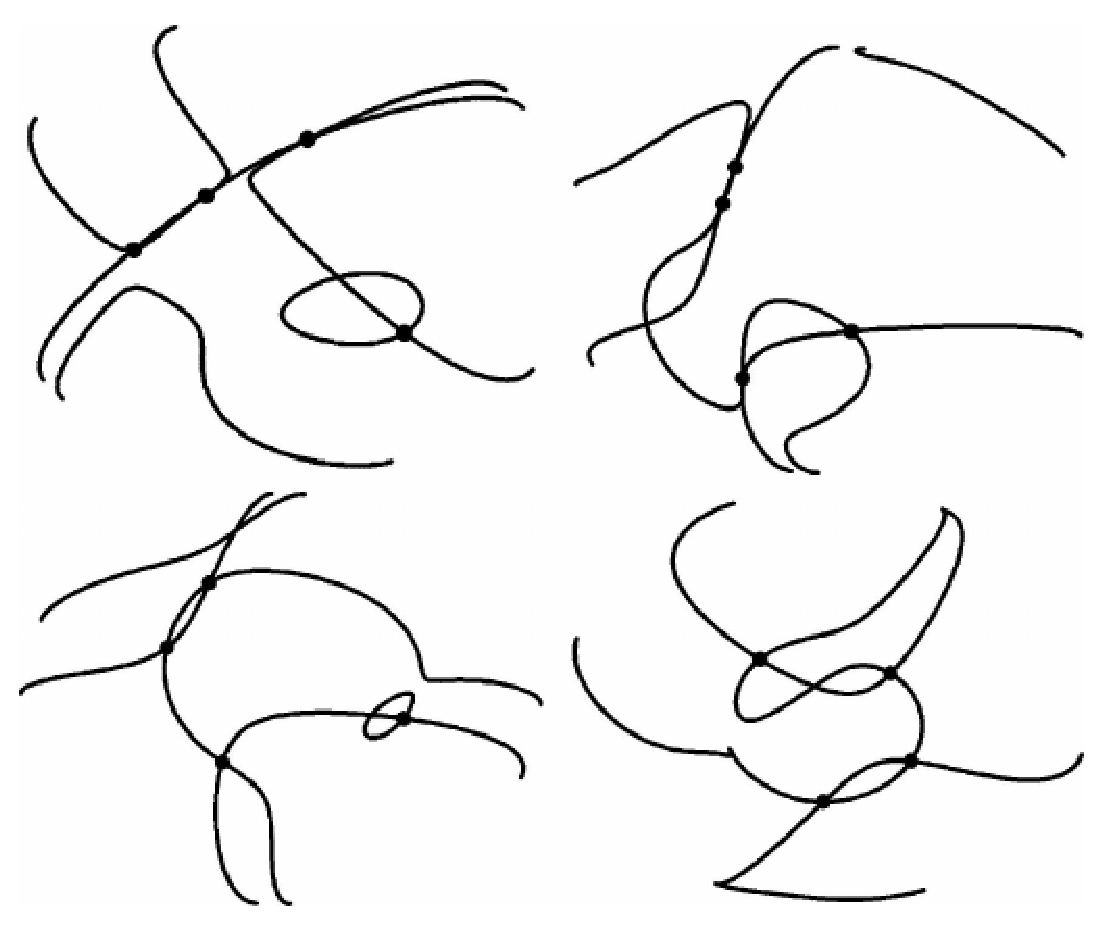
\includegraphics[scale=.85]{ex-curva-10}
\caption{\textit{Quatro exemplos de curvas de decimo grau definidas pela equaçao \ref{dez}, juntamente com seus respectivos epipolos.}}
\label{curva-10}
\end{figure}

Dado um ponto na curva de décimo grau, é importante verificar se o mesmo satisfaz a restrição de orientação, que é o fato de o correspondente ponto 3D no espaço situar-se em frente ao plano das duas imagens, conforme retratado na figura \ref{retr-orien}. Ou seja, o ponto no espaço 3D deve situar-se na metade da frente dos raios emanados de seus respectivos pontos nas duas imagens. Dado um epipolo ${\bf e}$ numa imagem, ${\bf e'}$ fica unicamente determinado pela equação \ref{funcao-de-e} na outra imagem. Após determinado o par de epipolos, a homografia da linha epipolar é unicamente definida pela correspondência desses pontos e assim determinamos a matriz essencial. Se ignorarmos uma diferença de escala considerando que a linha base que liga as duas câmeras tem comprimento unitário, temos que existem quatro configurações para a posição das duas imagens num sistema 3D. A restrição projetiva é satisfeita em quisquer dessas quatro configurações, pois os dois raios emanados do par de pontos correspondentes nas duas imagens continuam coplanares e devem se interseptar num ponto comum. A restrição de orientação é satisfeita exatamente quando os quatro pares de pontos correspondentes indicam a mesma configuração. Podemos dividir a restrição de orientação em duas partes: primeiro quando a homografia de reta epipolar é orientada, ou seja, quando os dois raios passando pelo par de pontos correspondentes nas imagens, estão no mesmo semiplano definido pela reta base onde se encontram as imagens (será chamada restrição de orientação epipolar); e segundo, a condição de que as duas metades dos raios que se projetam para a parte da frente devem convergir para um ponto comum (será chamada restrição de convergência).  

\begin{figure}[!htb]
\centering
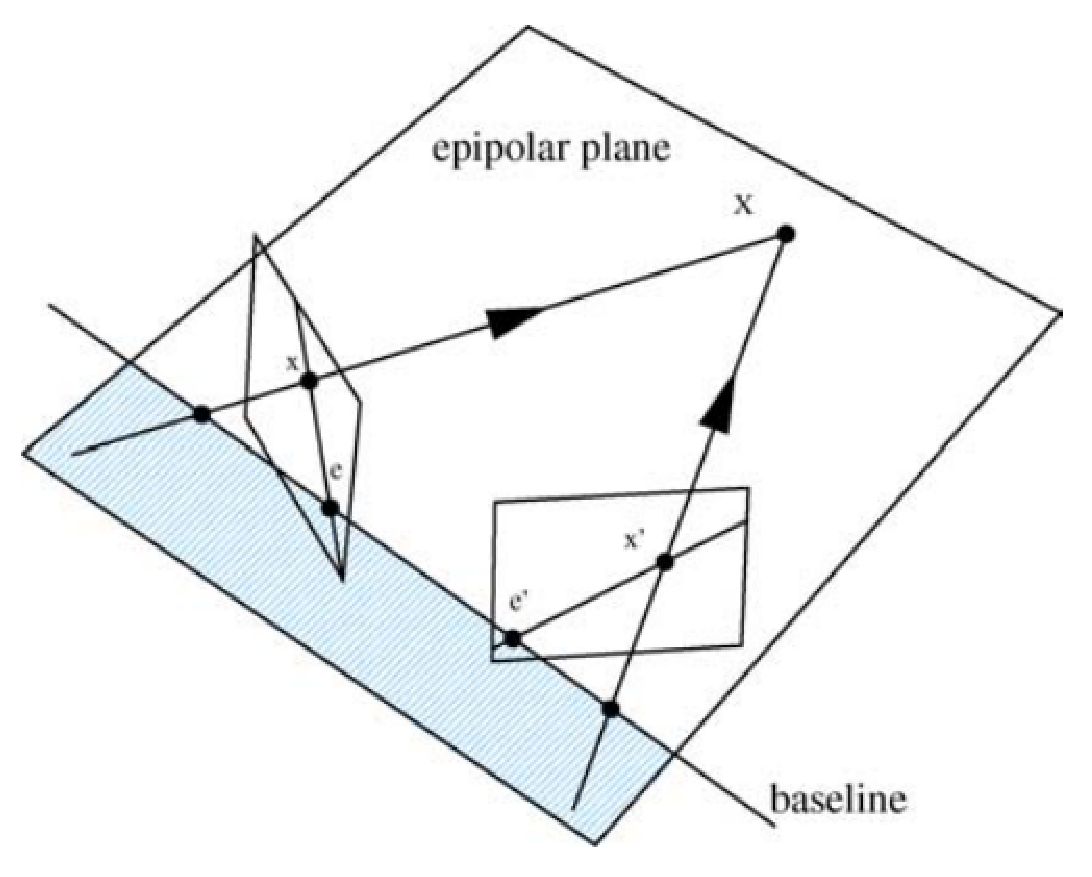
\includegraphics[scale=.85]{restricao-orientacao}
\caption{\textit{A restrição de orientação é simplesmente o fato de que o ponto no espaço 3D deve estar na parte da frente dos respectivos raios emanados de cada imagem.}}
\label{retr-orien}
\end{figure}

A restrição de convergência deve garantir que raios retroprojetados de cada imagem devem convergir. Isso não acontece somente se os raios forem paralelos e, uma forma de parametrizar, é através do ângulo formado entre o ponto na primeira imagem ${\bf x}$ e ${\bf e}$, e o ângulo entre o ponto na segunda imagem ${\bf x'}$ e ${\bf e'}$. Como a reta base passa por ${\bf e}$ e ${\bf e'}$, se os ângulos com os respectivos pontos forem iguais, os dois raios serão paralelos e não ocorrerá a convergência.


{\bf Aplicação da teoria no caso trifocal, com quatro pontos e três imagens.} As novidades do artigo se encontram, basicamente, no tipo de reconstrução 3D para duas imagens. A aplicação a seguir segue o padrão, até então convencional, de projetar as reconstruções na terceira imagem e minimizar o erro em relação aos dados já disponíveis. Assim, dados quatro pontos numa imagem e suas respectivas correspondências em outras duas imagens (todas com as câmeras calibradas), podemos escolher duas dessas imagens para traçarmos a curva de décimo grau de acordo com a esolha de um parâmetro $\theta$ que irá definir a cônica $B$, do feixe de cônicas, a ser utilizada.  Dada $B$ podemos calcular a cônica $G$ a partir da equação \ref{conica-G} como uma função de $B$, e as interseções de $B$ e $G$ podem ser determinadas como a solução de uma equação de quarto grau confrome descrito no apêndice do artigo. Assim, temos quatro soluções para   ${\bf e}$ e cada solução pode ser usada para calcular ${\bf e'}$ na segunda imagem de acordo com a equação \ref{funcao-de-e}. Note que para cada parâmetro $\theta$ teremos, a partir daqui, dezesseis caminhos a seguir. Com os epipolos encontramos a homografia da reta epipolar  e daí, a matriz essencial das duas imagens para cada uma das soluções. Existem vários métodos para reconstrução à partir da triangulação usando duas imagens, como por exemplo, \cite{nister5p2v} e \cite{Fabbri:Kimia:IJCV2015}. Conseguidas as reconstruções dos pontos 3D, existem também vários outros métodos de obtenção da câmera ralativa à terceira imagem, como por exemplo \cite{haralick} e \cite{bib:kuang}. Usados três pontos 3D para determinar a câmera da terceira imagem, podemos usar o quarto ponto para ser projetado na terceira imagem e comparar o resultado com o dado já obtido. Ou seja, para cada escolha do parâmetro $\theta$ (ou da cônica $B$), o procedimento consiste em minimizar um erro na imagem. Como o problema é supra restringido por um grau de liberdade, com os ruídos das correspondências, o valores encontrados para a reprojeção do quarto ponto não coincidirá com o dado observado mesmo que usada a correta solução. Como para cada $\theta$ escolhido teremos dezesseis configurações de câmera da terceria imagem e dezesseis reporjeções, todas essas reprojeções definem uma complexidade enorme de curvas na terceira imagem. Na figura \ref{curvas-f(theta)} é dada uma ideia da dificuldade extrema do problema envolvendo três imagens e quatro pontos. 

\begin{figure}[!htb]
\centering
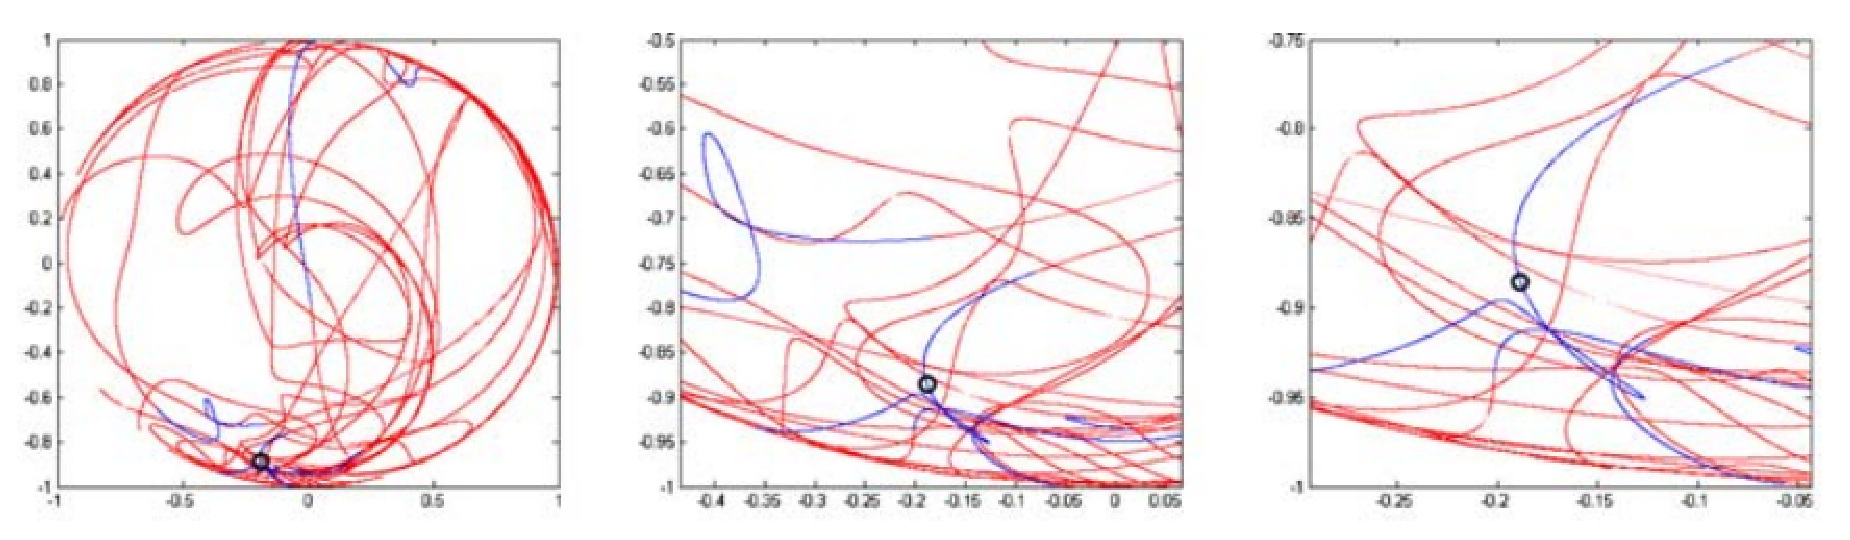
\includegraphics[scale=.52]{varias-curvas-f-theta}
\caption{\textit{A reprojeçao do feixe de conicas na terceira imagem e do quarto ponto reconstruido nos da uma ideia da dificuldade do problema de 3 imagens com quatro pontos.}}
\label{curvas-f(theta)}
\end{figure}

Para um grupo aleatório de quatro pontos, em geral a projeção da curva de décimo grau não passará pelos pontos. Antes de iniciar os cálculos, os pontos são co-registrados por uma homografia que será usada para transformar o DIAC  da segunda imagem no sistema de coordenadas da primeira. Existem várias maneiras de parametrizar o feixe de cônicas e uma delas é escolher duas cônicas dentre as degeneradas como base para o feixe.



%\section{Geometria Diferencial Trifocal}\label{sec:geo:dif:tri}

\subsection{Abordagem do Fabbri}
Problema 2.

\subsection{Nova Solução}

\subsection{Novo Algoritmo}

\subsection{Experimentos com novo Algoritmo}



%\section{Aplicações da Geometria Diferencial Trifocal}
(Objetivo: apanhado geral do uso de geometria trifocal e ideias novas)

\subsection{Aplicações em Sistemas de SfM}
Aplicações em structure for motion.

Explicar como utilizar os resultados dos dois últimos capítulos em sistema real.

\subsection{Outras Aplicações}
%\input{expe_conc}
%\section{Conclusões}

Existe toda uma engenhosidade no emprego de coordenadas homogêneas para fazer com que uma transformação projetiva funcione como uma transformação linear, mesmo que exista (disfarçadamente) a aplicação de uma translação. Além disso, a representação de pontos em coordenadas homogêneas favorece a representação de objetos algébricos abstratos, como pontos no infinito e a cônica absoluta, e a dedução de propriedades não existentes em outras geometrias, como a interseção de retas paralelas.

As pesquisas em visão computacional são auxiliadas por outras áreas da matemática aparentemente desconexas da geometria projetiva, pois na seção \ref{sec.astrom} verificamos a utilização do Quatérnion de Hamilton para parametrizar uma matriz de rotação e das Bases de Gr\"obner e Matriz de Ação na solução de sistemas de equações polinomiais, ambos empregados na determinação de uma câmera $P$. A própria utilização de sistemas de equações polinomiais com muitas variáveis na modelagem de problemas atuais pode se constituir uma novidade para vários pesquisadores.

Constatamos na seção \ref{sec.geo-tri} alguns benefícios do uso do tensor trifocal num sistema com três imagens em detrimento do uso puramente da geometria epipolar. Há a diminuição de alguns casos de degeneração para a correspondência de pontos em três imagens, e há também o benefício da determinação direta de uma reta numa imagem dadas as retas correspondentes nas outras duas imagens. Não há equação para a transferência direta de retas usando apenas geometria epipolar.

O estudo da geometria trifocal envolve uma quantidade grande de conhecimento da teoria básica de geometria projetiva conforme vimos na seção \ref{sec.nister}. Mais ainda, estudar geometria trifocal em problemas de reconstrução requer o conhecimento também da geometria epipolar, não somente em termos de comparação sobre qual das abordagens funciona melhor para reconstrução, mas também para entendermos de que forma a geometria epipolar pode ser útil num sistema com três imagens. Ficou clara a complexidade da tarefa de se determinar as três câmeras num sistema trifocal, e fazer essa determinação em termos de geometria diferencial é uma das fronteiras em visão computacional. 


\nocite{Fabbri:Kimia:CVPR10,Hartley2004,Faugeras,Schmid00,2503343,HartleyLi,koser,kukelova,pajdla,byrod}


\appendix
\section{Alguns Conceitos e Definicoes em Algebra Linear}
Esta secao do apendice se destina a apresentar algumas ferramentas da algebra linear necessarias ao entendimento de algumas secoes da dissertacao, funcionando como complementacao dessas secoes.

\subsection{A Matriz Anti-Simétrica $[{\bf v}]_\times$}
Dado um vetor ${\bf v}=(v_1,v_2,v_3)^\top$ é possível construir uma matriz anti-simétrica com as componentes de ${\bf v}$ na forma

\begin{equation*}
[{\bf v}]_\times=
\begin{bmatrix}
0&-v_3&v_2\\
v_3&0&-v_1\\
-v_2&v_1&0
\end{bmatrix},
\end{equation*}
onde a notação $[{\bf v}]_\times$ indica o produto vetorial entre um vetor qualquer ${\bf u}$ e ${\bf v}$. 

\begin{equation*}
{\bf v} \times {\bf u} = [{\bf v}]_\times {\bf u} = ({\bf v}^\top [{\bf u}]_\times)^\top
\end{equation*}

Sabemos que o produto vetorial entre um vetor e ele mesmo é sempre o vetor nulo, portanto o vetor ${\bf v}$ é o vetor nulo à direita e à esquerda de $[{\bf v}]_\times$. Desta forma, esta matriz anti-simétrica será sempre definida por seu vetor nulo.  

\subsection{A Pseudo-Inversa de $P$}

\newpage
\section{Alguns conceitos e definições de geometria algébrica}\label{sec.geo-algebrica}

Esta seção se destina a apresentar um resumo das definições básicas em Geometria Algébrica, bem como alguns conceitos e definições mais avançados necessários ao entendimento do procedimento de solução de sistemas de equações polinomiais. Para acessar um detalhamento maior da teoria juntamente com as demonstrações dos teoremas, o leitor pode consultar os livros \citep{cox-using} e \citep{cox-ideals}.

\subsection*{Definições básicas}

A Geometria Algébrica tem como objetivo principal de estudos as variedades algébricas, os objetos geométricos
formados pelos pontos que são soluções de um sistema de equações polinomiais. Para realizar esse estudo, utiliza técnicas de álgebra comutativa em conjunto com a linguagem geométrica.

{\it Monômios} são o produto de $n$ variáveis da forma $x_1^{\alpha_1}\cdot x_2^{\alpha_2} \cdot ... \cdot x_n^{\alpha_n}$ onde os expoentes são números inteiros não-negativos. O grau total de um monômio é a soma dos expoentes das variáveis e é denotado por $|\alpha|=\alpha_1+\alpha_2+...+\alpha_n$, e para simplificar a notação é adotada a convenção onde $\alpha=(\alpha_1,\alpha_2,...,\alpha_n)$ é o vetor dos expoentes e $x^\alpha=x_1^{\alpha_1}\cdot x_2^{\alpha_2} \cdot ... \cdot x_n^{\alpha_n}$ é a representação do monômio.

{\it Polinômios} são combinações lineares dos monômios denotados por
\begin{equation*}
f=\sum_\alpha a_\alpha x^\alpha,\quad\text{onde}\quad a_\alpha\in k.
\end{equation*} 
Os coeficientes desses polinômios pertencem a um conjunto numérico denominado {\it corpo}, denotado por $k$, que pode ser o conjunto dos números complexos ou reais, por exemplo. Informalmente, corpo é um conjunto fechado para adição, subtração, multiplicação e divisão com suas propriedades usuais. O conjunto de todos os polinômios nas $n$ variáveis definidas num corpo $k$ é denotado por $k[x_1,...,x_n]$.

Se estivermos trabalhando com pouca variáveis podemos utilizar $x$, $y$ e $z$ e como exemplo temos
\begin{equation*}
f=2x^3y^2z+\frac{2}{3}y^3z^3-3xyz+y^2\quad\in\quad\mathbb{Q}[x,y,z],
\end{equation*} 
onde
\begin{itemize}
\item os {\it coeficientes} são 2, $\frac{2}{3}$, -3 e 1,
\item os {\it termos} são cada monômio junto com o respectivo coeficiente
\item o {\it grau total} do polinômio é o grau do monômio de maior grau; no caso temos dois monômios com grau 6.
\end{itemize}

A soma e o produto de dois polinômios também são polinômios, mas um polinômio $f$ divide um polinômio $g$ apenas se existe um polinômio $h$ onde $g=f\,h$. Assim, entre polinômios ficam satisfeitos os axiomas de adição e multiplicação em um corpo, mas não a existência de um inverso multiplicativo, pois por exemplo, $f=\frac{1}{x}$ não é um polinômio. Os elementos que obedecem essa estrutura formam um {\it anel comutativo}, com estudos feitos com base na {\it álgebra comutativa}, e por isso o conjunto $k[x_1,...,x_n]$ é chamado {\it anel de polinômios}.

\subsection*{Ideal e variedade}
Um espaço $n$-dimensional num corpo $k$ é definido como
\begin{equation*}
k^n=\{(a_1,...,a_n)\,/\, a_1,...,a_n\in k\},
\end{equation*}
e é possível relacionar polinômios com um espaço $n$-dimensional observando que um polinômio nos dá uma função
\begin{equation*}
f:k^n\rightarrow k\quad\text{com}\quad f=\sum_\alpha a_\alpha x^\alpha\quad \in\quad k[x_1,...,x_n].
\end{equation*}
A capacidade em tratar polinômios como funções é o que possibilita ligar álgebra e geometria através das chamadas {\it variedades}, definida a seguir e denotada por ${\bf V}$.
\begin{equation*}
{\bf V}(f_1,...,f_s)=\{(a_1,...,a_n)\in k^n/\, f_i(a_1,...,a_n)=0, \,\forall\,\, 1\le i\le s\}.
\end{equation*}
Portanto, variedades podem ser entendidas como o conjunto de vetores que são solução de um sistema de equações polinomiais, e que fornecem uma representação geométrica para a solução do sistema sempre que possível.

Como exemplo, temos na figura \ref{fig.variedades} a representação geométrica das variedades ${\bf V}(xy-x^3+1)$ e ${\bf V}(-x^2-y+z)$, onde cada ponto no plano e no espaço é representado pelas soluções de $xy-x^3+1=0$ e $-x^2-y+z=0$, respectivamente.
\begin{figure}[!htb]
\centering
\subfloat[]{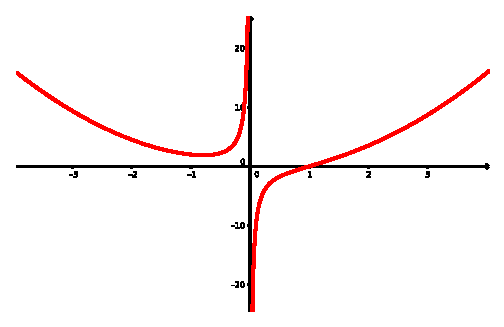
\includegraphics[scale=1]{variedade-1}}
\quad
\subfloat[]{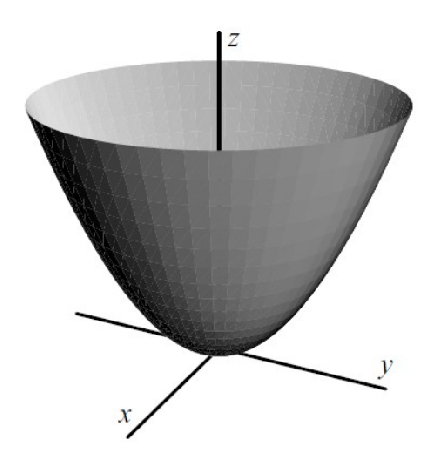
\includegraphics[scale=.8]{variedade-3D}}
\caption{{As representações geométricas podem ser obtidas usando as funções ({\tt a}) $y=\frac{x^3-1}{x}$ e ({\tt b}) $z=x^2+y$}.}
\label{fig.variedades}
\end{figure} 

{\it Ideal} é um subconjunto de $k[x_1,...,x_n]$ denotado por $I$ que satisfaz as condições:
\begin{itemize}
\item $0\in I$;
\item $f,g\,\in I \Rightarrow (f+g)\in I$;
\item $f \in I$ e $h \in k[x_1,...,x_n] \Rightarrow h\,f \in I$. 
\end{itemize}

Se $f_1,...,f_s$ são polinômios em $k[x_1,...,x_n]$ então podemos definir um ideal através desses polinômios que são chamados de {\it base} do ideal, usando a notação
\begin{equation*}
I=\left\langle f_1,...,f_s \right\rangle = \{\sum_{i=1}^s h_if_i\,:\,h_1,...,h_s \in k[x_1,...,x_n]\}.
\end{equation*}
Por exemplo, para sabermos se o polinômio $x^2-2x+2-y$ pertence ao ideal $\left\langle x-1-t\,,\,y-1-t^2 \right\rangle$ devemos verificar se é possível escrevê-lo como combinação das bases desse ideal, 
\begin{equation*}
x^2-2x+2-y=(x-1+t)(x-1-t)+(-1)(y-1-t^2).
\end{equation*}

Um mesmo ideal pode ser formado por bases diferentes e, quando isso acontece, as variedades definidas por cada base também são iguais, ou seja
\begin{equation*}
\left\langle f_1,...,f_s \right\rangle = \left\langle g_1,...,g_s \right\rangle \Rightarrow {\bf V}(f_1,...,f_s)={\bf V}(g_1,...,g_s).
\end{equation*}
Por exemplo, temos a seguir um ideal formado por bases diferentes (podemos verificar que se trata do mesmo ideal escrevendo os polinômios da esquerda como combinação dos polinômios da direita e reciprocamente) e que possuem variedades iguais:
\begin{equation*}
\left\langle 2x^2+3y^2-11\,,\,x^2-y^2-3 \right\rangle = \left\langle x^2-4\,,\,y^2-1 \right\rangle,\,\, \text{logo}
\end{equation*}
\begin{equation}\label{eq.variedades}
{\bf V}(2x^2+3y^2-11\,,\,x^2-y^2-3)={\bf V}(x^2-4\,,\,y^2-1)=\{(\pm2,\pm1)\}.
\end{equation}
Observe que todos os polinômios de um ideal terão o mesmo conjunto variedade gerado pelos polinômios da base. Observe ainda, que a base de um ideal pode ser pensada como um sistema de equações polinomiais, e que para encontrarmos o conjunto solução do sistema (variedade) podemos converter a base dada numa base mais simples conforme a relação \ref{eq.variedades}. Mais à frente veremos que é exatamente esse o procedimento realizado pelas bases de Gr\"obner.

\subsection*{As bases de Gr\"obner}

Para sabermos se um polinômio $f$ pertence a um ideal devemos dividir $f$ pelas bases do ideal e verificar se o resto é zero, pois assim $f$ pode ser escrito como combinação dos polinômios da base. Na divisão de polinômios de uma variável o resto é único, mas para polinômios de mais de uma variável, tanto o resto como os quocientes podem variar dependendo da ordem dos divisores e da ordenação de monômios escolhida ({\it lexicográfica, lexicográfica graduada e lexicográfica graduada reversa}). Para detalhes sobre divisão de polinômios de várias variáveis consultar \citep{cox-ideals}. 

Por exemplo, vamos verificar se o polinômio $f=xy^2-x$ pertence ao ideal $I=\left\langle xy+1\,,\,y^2-1 \right\rangle$. Efetuando a divisão de $f$ por $\{xy+1\,,\,y^2-1\}$ nesta ordem, obtemos
\begin{equation*}
xy^2-x=y(xy+1)+0(y^2-1)+(-x-y)
\end{equation*}  
com resto $-x-y$. Mas efetuando a divisão na ordem $\{y^2-1\,,\,xy+1\}$ teremos
\begin{equation*}
xy^2-x=x(y^2-1)+0(xy+1)+0
\end{equation*} 
com resto zero. Assim, $f\in I$ e vemos que, dada uma base qualquer de $I$, o resto zero é uma condição suficiente para que $f\in I$ mas não é uma condição necessária. 

Precisamos de uma base que facilite verificar se um polinômio pertence a um ideal, e as bases de Gr\"obner tem essa propriedade, pois um polinômio $f$ quando dividido pelas bases de Gr\"obner deixa resto único, não importanto a ordem dos divisores (base do ideal). Assim, sendo $G=\{g_1,...,g_t\}$ uma base de Gr\"obner, então 
\begin{equation*}
f\in I \Leftrightarrow \text{o resto da divisão de $f$ por $G$ é zero}.
\end{equation*}
Essa propriedade é tão importante que às vezes é tomada como a própria definição para as bases de Gr\"obner. O resto da divisão de um polinômio $f$ por $G=\{g_1,...,g_t\}$ é denotado por $\overline{f}^G$. Por exemplo, dividindo $f=x^5y$ por $G=\{x^2y-y^2\,,\,x^4y^2-y^2\}$ é $\overline{x^5y}^G=xy^3$, pois
\begin{equation*}
x^5y=(x^3+xy)(x^2y-y^2)+(0)(x^4y^2-y^2)+xy^3.
\end{equation*}
Para verificarmos se uma base é uma base de Gr\"obner utilizamos o {\it critério de Buchberger}, e caso não seja, toda base de um ideal pode ser convertida numa base de Gr\"obner utilizando o {\it algoritmo de Buchberger}. 

\subsection*{Resolvendo sistemas com as bases de Gr\"obner}

Considere o sistema
\begin{empheq}[left=\empheqlbrace]{align*}
x^2+y^2+z^2&=1\\
x^2+z^2-y&=0\\
x-z&=0,
\end{empheq}
cujas soluções podem ser obtidas como a extração do conjunto variedade do ideal
\begin{equation*}
I=\left\langle x^2+y^2+z^2-1\,,\,x^2+z^2-y\,,\,x-z\right\rangle. 
\end{equation*}
Como toda base de um ideal pode ser convertida numa base de Gr\"obner, aplicando o algoritmo de Buchberger calculamos uma nova base para o ideal
\begin{equation*}
I=\left\langle x-z\,,\,-y+2z^2\,,\,z^4+\frac{1}{2}z^2-\frac{1}{4}\right\rangle. 
\end{equation*}
Como um ideal com bases diferentes possui o mesmo conjunto variedade, podemos converter as bases de Gr\"obner num novo sistema que terá o mesmo conjunto solução do anterior,
\begin{empheq}[left=\empheqlbrace]{align*}
x-z&=0\\
-y+2z^2&=0\\
z^4+\frac{1}{2}z^2&=\frac{1}{4}.
\end{empheq}

Note que a última equação do sistema depende apenas de uma variável, que pode ser obtida através de um método numérico. O {\it teorema da eliminação} garante que, definida uma ordenação de monômios, as variáveis de um sistema são eliminadas de acordo com a precedência dessa ordem. Depois de calculada a primeira variável, por retro-substituição podemos determinar o valor das variáveis restantes, onde tal retro-substituição é garantida, sob determinadas condições, pelo {\it teorema da extensão}. Alguns softwares de computação algébrica (como Maple) possuem pacotes para computação das bases de Gr\"obner. O procedimento apresentado aqui para solução de sistemas possui algumas deficiências que serão comparadas com o procedimento a seguir no final do apêndice.

\subsection*{Álgebra de um espaço dimensional finito}

Na divisão de um polinômio $f\in k[x_1,...,x_n]$ por uma base de Gr\"obner $G$ obtemos a expansão
\begin{equation*}
f=h_1g_1+...+h_tg_t+\overline{f}^G,
\end{equation*} 
onde $\overline{f}^G$ é uma combinação de monômios que não são divisíveis pelos termos líderes dos polinômios de $G$. Mas existem outros polinômios em $k[x_1,...,x_n]$ que deixam o mesmo resto que $f$ na divisão por $G$. Assim $f$ definde uma {\it classe de equivalência} dada por
\begin{equation*}
[f]=\{p\in k[x_1,...,x_n]\,/\,p\equiv f\, \text{mod}\, I\}.
\end{equation*}
Ou seja, assim como temos os polinômios que pertencem ao ideal $I$, temos também o conjunto dos polinômios que não pertencem ao ideal, e cada um desses polinômios pertence à sua classe de equivalência. O conjunto de todas as classes de equivalência de um ideal forma um anel denominado {\it anel quociente}, denotado por
\begin{equation*}
k[x_1,...,x_n]/I=\{[f]\,/\,f\in k[x_1,...,x_n]\}.
\end{equation*}

Quando multiplicamos dois restos de um ideal, $\overline{f}^G\cdot\overline{p}^G$, podemos obter um polinômio que pertence ao ideal, mas quando somamos dois restos ou multiplicamos um resto por um escalar, o polinômio gerado continua pertencendo ao anel quociente $k[x_1,...,x_n]/I$. Por essa e outras características, temos que esse anel tem a estrutura de um {\it espaço vetorial} e é denominado {\it Álgebra}. Os monômios que não são divisíveis pelos termos líderes de $G$ formam uma base para essa Álgebra, denominada {\it base linear}. Considere como exemplo o ideal gerado por 
\begin{equation}\label{eq.base-G}
G=\{x^2+\frac{3xy}{2}+\frac{y^2}{2}-\frac{3x}{2}-\frac{3y}{2}\,,\,xy^2-x\,,\,y^3-y\},
\end{equation}
cujo polinômios têm os termos líderes dados por $\{x^2\,,\,xy^2\,,\,y^3\}$. Extraindo os monômios que não são divisíveis pelos termos líderes formamos a base linear
\begin{equation*}
B=\{1\,,\,x\,,\,y\,,\,xy\,,\,y^2\},
\end{equation*}
onde os cinco monômios são uma base do espaço vetorial para a álgebra $A={\mathbb C}[x,y]/I$. Assim, todo polinômio que não pertence a $I$ pode ser escrito como uma {\it combinação linear} dos monômios de $B$.

A base linear $B$ tem dimensão finita e sempre terá desde que sejam satisfeitas as condições do {\it teorema da finitude}, para o qual a principal condição é que sendo $G$ uma base de Gr\"obner para um ideal $I \subset k[x_1,...,x_n]$, então para cada $1\le i\le n$, existe um $m_i\ge 0$ tal que $x_i^{m_i}$ é o termo líder de algum $g\in G$. Ou seja, considerando a base $G$ na relação \ref{eq.base-G}, se por exemplo $y^{m_y}$ não pertencesse ao conjunto dos termos líderes para algum $m_y$, não teríamos um expoente que pudesse restringir $y$ a pertencer à base $B$, e esta seria infinita.

\subsection*{Resolvendo sistemas com autovalores e autovetores}

A ideia principal é explorar a estrutura de $A=k[x_1,...,x_n]/I$ para estimar o valor de alguma funcão $f$ nos valores de $V$. Observe que nossa tarefa é encontrar os valores de $x_i\in (x_1,...,x_n)$ onde $(x_1,...,x_n)\in V$, assim podemos tomar a função $f=x_i$, pois estimar o valor para $f$ cumprirá a tarefa de encontrar os valores de cada componente do vetor solução.

Para determinar o valor de cada variável é definido um operador linear $m_{x_i}$ como a multiplicação de cada variável $x_i$ pelos polinômios $b$ da base $B$.
\begin{equation*}
m_{x_i}:A\rightarrow A\quad\text{onde}\quad m_{x_i}([b])=x_i\cdot[b].
\end{equation*} 
Desta forma, os possíveis valores para a variável $x_i$ são computados através da decomposição em autovalores da matriz $m_{x_i}$. Por definição em Álgebra Linear, para encontrarmos a matriz $m_{x_i}$,  devemos expandir $p_j=x_i\cdot b_j$ em termos da base $B$, e tomar a transposta da matriz dos coeficientes dessa expansão.

Contudo, multiplicando dois elementos de $A$, não podemos garantir que o resultado $p_j$ seja um elemento de $A$ que possa ser escrito como combinação linear dos elementos de $B$. Assim, devemos escrever a expansão de $p_j$ em termos dos elementos da base $G$ para obter o resto $\overline{p}^{G}$. Como todo polinômio
\begin{equation}\label{eq.resto-mod}
p\equiv\overline{p}^{G}\,\text{mod}\,I,
\end{equation} 
podemos expandir $\overline{p}^{G}$ ao invés de $p$. 

Como exemplo, vamos calcular as soluções do sistema formado pelos polinômios da base $G$ em \ref{eq.base-G},
\begin{empheq}[left=\empheqlbrace]{align*}
x^2+\frac{3xy}{2}+\frac{y^2}{2}-\frac{3x}{2}-\frac{3y}{2}&=0\\
xy^2-x&=0\\
y^3-y&=0,
\end{empheq}
com termos lideres $\{x^2\,,\,xy^2\,,\,y^3\}$ e base $B=\{1\,,\,x\,,\,y\,,\,xy\,,\,y^2\}$. Determinando primeiramente os valores para $x$ temos que $m_x(b_j)=x\cdot b_j$, portanto
\begin{equation*}
\begin{array}{rcccl}
x\cdot1 &= &x& = &0 \cdot 1 + 1 \cdot x + 0 \cdot y + 0 \cdot xy + 0 \cdot y^2\\\\
x \cdot x &= &x^2&=& 0 \cdot 1 + \frac{3}{2} \cdot x + \frac{3}{2} \cdot y - \frac{3}{2} \cdot xy\, – \,\frac{1}{2} \cdot y^2\\\\
x \cdot y &=& xy &= &0 \cdot 1 + 0 \cdot x + 0 \cdot y + 1 \cdot xy + 0 \cdot y^2\\\\
x \cdot xy &=& x^2y &= &0 \cdot 1\, – \,\frac{3}{2} \cdot x \,–\, \frac{1}{2} \cdot y + \frac{3}{2} \cdot xy + \frac{3}{2} \cdot y^2\\\\
x \cdot y^2 &= &xy^2& =& 0 \cdot 1 + 1 \cdot x + 0 \cdot y + 0 \cdot xy + 0 \cdot y^2.
\end{array}
\end{equation*}
Tomando a transposta dos coeficientes temos a denominada {\it matriz de ação},
\begin{equation*}
m_x=
\begin{bmatrix}
0&0&0&0&0\\\\
1&\frac{3}{2}&0&-\frac{3}{2}&1\\\\
0&\frac{3}{2}&0&-\frac{1}{2}&0\\\\
0&-\frac{3}{2}&1&\frac{3}{2}&0\\\\
0&-\frac{1}{2}&0&\frac{3}{2}&0
\end{bmatrix},
\end{equation*}
e os valores para $x$ são dados pelos autovalores $\{-1,2,1,1,0\}$, que podem ser calculados usando o método em \ref{sec.potencias-autovalores}.
 De forma análoga, podemos determinar os valores de $y$ através dos autovalores $\{1,-1,1,-1,0\}$ de $m_y$. As soluções do sistema é o conjunto variedade do ideal $I$ que tem como base $G$,
 \begin{equation*}
 V(I)=\{(-1,1),(2,-1),(1,1),(1,-1),(0,0)\}.
 \end{equation*}

Podemos ver que na expansão de $x\cdot b_j$ acima, os monômios $\{x^2\,,\,x^2y\,,\,xy^2\}$ não podem ser escritos como combinação linear da base $B$. Por isso, usando a propriedade em \ref{eq.resto-mod}, fizemos a expansão do resto da divisão de cada um desses monômios pela base $G$,
\begin{equation*}
\begin{array}{rcl}
\overline{x^2}^{G}&=&-\frac{3xy}{2}-\frac{y^2}{2}+\frac{3x}{2}+\frac{3y}{2}\\\\
\overline{x^2y}^{G}&=&\frac{3xy}{2}+\frac{3y^2}{2}-\frac{3x}{2}-\frac{y}{2}\\\\
\overline{xy^2}^{G}&=&x.
\end{array}
\end{equation*}

É possível determinar o conjunto variedade usando a retro-substituição ou a matriz de ação. Vejamos as principais diferenças:
\begin{itemize}
\item O método da eliminação impõe o uso da ordenação
lexicográfica, a qual requer muita computação e, mesmo usando um algoritmo para mudança de ordenação, não é eficiente. A estrutura algébrica de $A={\mathbb{C}}[x_1,...,x_n]/I$
é independente de quaisquer das três ordenações de monômios escolhida, assim qualquer tipo de ordenação pode ser utilizada no cálculo dos operadores $m_{x_i}$.
\item Computação numérica versus computação simbólica, e instabilidade numérica. As entradas das matrizes $m_{x_i}$ sempre são números racionais e podem ser determinadas, exatamente, por
computação simbólica. Assim, a computação numérica fica restrita somente ao cálculo dos
autovalores.
\item  Podemos computar as matrizes $m_{x_i}$ 
 e seus autovalores separadamente e determinar os
vetores $(x_1,...,x_n)$
 que dão as soluções aproximadas. Ou seja, o cálculo da variável $x_j$
não depende do cálculo da variável $x_i$
 como na eliminação. Isso resolve um dos maiores problemas na retro-substituição, o problema dos {\it erros acumulados}.

\item É possível reduzir o esforço computacional mais ainda calculando os autovalores de uma única matriz de ação $m_{c_1x_1+...+c_nx_n}$.

\end{itemize}
\newpage











%\section{Possiveis Publicacoes}
%\subsection{Trifocal Relative Pose using First-Order Differential Geometry}
%Paper mais importante onde resolveriamos o problema para pontos e tangentes.
%
%Capitulos de tese: \ref{sec:geo:dif:tri}
%
%\subsection{Using Trifocal Geometry in Structure from Motion}
%Outros titulos:
%"Trifocal geometry: Theory and practice in real SfM systems"
%"Exploiting Trifocal geometry for bootstrapping SfM systems"
%"A Survey of Trifocal Geometry in Structure from Motion"
%
%Capitulos de tese: \ref{sec:apli:geo:dif:tri}
%
%Este responderia às seguintes perguntas:
%Qual a vantagem de se iniciar um sistema de autocalibracao externa de cameras usando
%geometria trifocal?  O que se ganha em reconstrucao/estereo?
%
%Experimentos:
%- implementar bundler com geometria trifocal e observar melhorias
	
\bibliographystyle{plainnat} 
\bibliography{biblio}
\end{document}
\grid
